\documentclass[a4paper,11pt]{report}
\usepackage[margin=2cm]{geometry}
\usepackage{listings}
\usepackage{amsmath}
\usepackage{amssymb}
\usepackage[table]{xcolor}
\usepackage{graphicx}
\usepackage{wrapfig}
\usepackage{algorithm}
\usepackage{algorithmicx}
\usepackage{algpseudocode}
\usepackage{bbm}
\usepackage{tikz}
\usepackage[skip=10pt, indent=0pt]{parskip}

%%%%%%%%TIKZ SUDOKU%%%%%%%%%%
\newcounter{row}
\newcounter{col}
\newcounter{rowa}
\newcounter{cola}
\newcounter{rowb}
\newcounter{colb}

\newcommand\setrow[9]{
  \setcounter{col}{1}
  \foreach \n in {#1, #2, #3, #4, #5, #6, #7, #8, #9} {
    \edef\x{\value{col} - 0.5}
    \edef\y{9.5 - \value{row}}
    \node[anchor=center] at (\x, \y) {\n};
    \stepcounter{col}
  }
  \stepcounter{row}
}
\newcommand\setrowa[4]{
  \setcounter{cola}{1}
  \foreach \n in {#1, #2, #3, #4} {
    \edef\x{\value{cola} - 0.5}
    \edef\y{4.5 - \value{rowa}}
    \node[anchor=center] at (\x, \y) {\n};
    \stepcounter{cola}
  }
  \stepcounter{rowa}
}
\newcommand\setrowb[3]{
  \setcounter{colb}{1}
  \foreach \n in {#1, #2, #3} {
    \edef\x{\value{colb} - 0.5}
    \edef\y{3.5 - \value{rowb}}
    \node[anchor=center] at (\x, \y) {\n};
    \stepcounter{colb}
  }
  \stepcounter{rowb}
}
%%%%%%%%%%%%%%%%%%%%%%%%

\author{E. Routledge}
\date{01 Nov 2022}
\title{Sudoku is Hard}


\begin{document}
\lstset{language=Python}
\input{titlepage}
\begin{center}{\huge\textbf{Plagarism Declaration}}\end{center}
\textit{This piece of work is a result of my own work except where it forms an assessment based on group project work. In the case of a group project, the work has been prepared in collaboration with other members of the group. Material from the work of others not involved in the project has been acknowledged and quotations and paraphrases suitably indicated.}
\begin{center}{\textbf{Abstract}}\end{center}

\tableofcontents
% ~~~~~~~~~~~~~~~~~~~~~~~~~~~~~~~~~~~~~~~~~~~~~~~~~~~~~~~~~~~~~~~~~~~~~~~~~~~~~~~~~~~~~~~~~~~~ %
\chapter{Introduction}

Sudoku is a simple logic game, in the standard $9 \times 9$ (or $3 \times 3 \times 3 \times 3$) one must complete the grid such that every row, column and box contains the numbers 1 to 9, that is all. For many, this is a brain teaser at the back of a newspaper or a game on their phone used to pass the time on a commute. So why are we bothered about the mathematics behind the game? The answer is multifaceted. 

Sudoku is a serious hobby for many and even a job. All major newspapers will have a sudoku section the New york times has three sudokus set each day (https://www.nytimes.com/puzzles/sudoku), these all need to be created and verified which is no easy task (not even for a computer as we shall soon find out). Then there are the freely available apps with thousands of sudokus of varying difficulty. Sudokus get so hard that there is even a world sudoku Championship (https://www.worldpuzzle.org/championships/wsc/) where teams and individuals compete to get the best time for a sudoku solve. In 2022 Mark Goodliffe came first in the WSCs over 50s challenge. This is significant as Mark is half of a duo creating entertaining videos on the solution of sudokus and its variants on the youtube channel Cracking the Cryptic (https://www.youtube.com/@CrackingTheCryptic). During the coronavirus pandemic this author spent many hundreds of hours learning techniques from Cracking the Cryptic and putting them into practise. With that said, sudoku provides many opportunities for revenue and by studying the mathematics behind this puzzle those jobs may be made easier.

- Mental Exercise 

The literature on the mathematics of sudoku is extensive and ranges through many different areas such as group theory, discrete mathematics, complexity theory and information theory all while being digestable for a undergraduate audience. Theory is best learnt through application so examining sudoku through these lenses can consolidate learning as well as encourage and motivate students to continue learning mathematics at a higher level. An excellent example of this is the book Taking Sudoku Seriously \cite{}, using sudoku as the catalyst many foundational maths ideas are made accessible to those who haven't studied mathematics past GCSE.

An exploration of sudoku also serves to unite the authors favourite subjects, mathematics and computer science. While it is known underlying knowledge of mathematics is required to study computer science, the opposite is not entirely obvious. Through our exploration of sudoku we link theory to tangible computation, for we often study theory in mathematics without regard for what it means in practise, the time taken to execute such mathematical processes is important it is the difference between trivial and the heat death of the universe. This author believes it important for mathematicians to have a grasp of such concepts and we use sudoku as the lens for motivating this. Discuss the lack of mathematical proof but evidence of success in AI.

Sudoku stems from magic and latin squares (more to be discussed later). Many variants have popped up from the original we have killer and thermo and this authors personal favourites are magic squares within a sudoku, feels very full circle. This is clearly a branching puzzle with no signs of stopping (see Cracking the Cryptic for new variants every week).

We can see that sudoku is not just a brain teaser, its popularity is ever expanding and its use for educational and monetary are self evident. So it makes sense to study the mathematical structure of sudoku.

\section{History}

Sudoku isnt as old as you think it is in fact the name sudoku only came about in 1986. It is seen in French newspapers from the 19th century but in different variations to the standard puzzle we know today, during this period it is named \textit{carre magique diabolique} refering to the magic square puzzles that were around as early as 190 BCE and can be seen in various art works over the centuries. So sudoku has a French origin as eventhough they are refered to as magic squares and do not mark the boxes within the sudoku, each subsquare did in fact contain the digits 1-9. Modern sudoku is thought to be first published in 1979, named Number Place. In 1984 the puzzle made its way to japan where a puzzle company trademarked the name we know today and enforced symmetrical puzzles (rotationally symmetry) for aesthetic reasons. Soon variants of sudoku with different box shapes started gaining popularity.

Magic squares are the ancestors of sudoku, these are $n$ by $n$ grids with numbers such that rows, columns and the two diagonals add up to the same value, termed the magic constant. These squares were known by mathematicians around the world and the first example of a 4th order ($n=4$) square occurred in India in 587 CE. Euler too worked with magic squares and left many open questions; the existance of a $3\times 3$ magic square comprising of square numbers.

Latin squares are another note worthy ancestor to the sudoku, this is a $n$ by $n$ grids with $n$ digits such that no digit repeats in the row or column of the grid. Sudokus are a version of latin squares but with an added box constraint. While the name is inspired by Euler, a  Korean mathematician in 1700 published an example of a Latin square, beating Euler by almost 70 years. 
	
\section{Defining Sudoku Notation}
	
\textbf{Def$^n$}: A $n$ by $n$ Sudoku puzzle $P$ is a function $P:  \{1,...,n\}^2\rightarrow\mathbb D \cup \{0\}$ where $\mathbb D$ is an alphabet of size $n$ most commonly $\mathbb D = \{1,...,n\}$, the $\{0\}$ represents the blank symbol. $P$ is usually displayed as a board and the blank symbol ommitted. There are three rules a valid sudoku puzzle follows, the row restriction, column restriction and box restriction.

The column restriction: for all $i,j,k\in \{1,...,n\}$ if $P(i,j)\neq0$ and $P(i,k)\neq0$ then $P(i,j)\neq P(i,k)$. This is to say: non blank values cannot be repeated in a column. When referencing columns we use C1,...,C$n$.

The row restriction: this is the same as the column restriction but applied to rows. For all $i,j,k\in \{1,...,n\}$ if $P(i,j)\neq0$ and $P(k,j)\neq0$ then $P(i,j)\neq P(k,j)$. We call rows in $P$ R1,...,R$n$.

Puzzles conforming to just the two above rules are named Latin squares. 

The box restriction: for $x\leq y$ such that $xy=n$ and for all $i,j,k,l\in\{1,...,n\}$ with $\lfloor \frac{j-1}{x} \rfloor=\lfloor \frac{l-1}{x}\rfloor$, $\lfloor \frac{i-1}{y} \rfloor=\lfloor \frac{k-1}{y}\rfloor$, $P(i,j)\neq0$ and $P(k,l)\neq0$ then $P(i,j)\neq P(k,l)$. We introduce box regions of size $x\times y$, these cannot have repeated values. We label these B1,..,B$n$ from left to right and top to bottom. Note we can enforce $x\leq y$. 

\textbf{Remark}: when $n$ is prime the box condition is the same as the row condition which reduces the sudoku puzzle to a latin square puzzle, therefore we omit these values of $n$. The most common sudokus are square numbers with boxes of size $\sqrt{n}$. If the box size is not stated then it is assumed to be the factor pair excluding 1 and $n$.

A few sudokus have specific names:
\begin{itemize}
\item Shidoku is $4\times 4$,
\item Rudoku is $6\times 6$ and
\item Sudoku without specification is $9\times 9$.
\end{itemize} 

\textbf{Def$^n$}: A completed sudoku puzzle does not have any blank symbols. $P:  \{1,...,n\}^2\rightarrow\mathbb D$ 

\textbf{Def$^n$:} A sudoku $P$ has a solution if there exists an augmentation of the puzzle such that blank symbols are changed to values from $\mathbb D$ and no other values of $P$ are changed.

\textbf{Def$^n$}: The set $P_n$ includes all complete sudoku grids with size $n$ by $n$, if $n$ has more than one factor pair that is not itself and 1 we have to specify the box size. For example when $n=12$ we have two sets $P_{2,6}$ and $P_{3,4}$. For cases where $n$ is a square number but has multiple factor pairs $P_n$ denotes the puzzles with $\sqrt{n}$ sized boxes.

\textbf{Def$^n$}: To aid us in describing positions on a board we use the following terminology: a cell is a single (i,j) location in $P$, a sash is the rows split into $y$ groups ($y$ from the box restriciton definition) enumerated S1,..,S$y$ and a tower is the coloums split into $x$ groups  ($x$ from the box restriciton definition) enumerated T1,..,T$x$.

\begin{figure}[h!]
	\begin{center}
		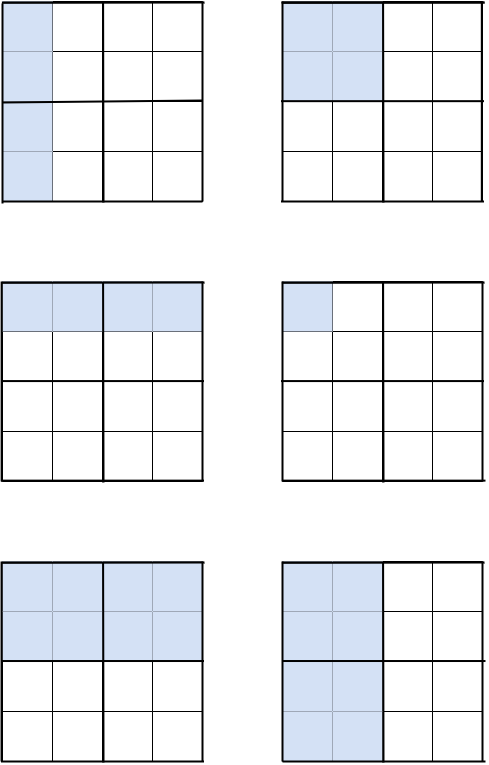
\includegraphics[width=50mm]{figures/highlighted_cells.png}
	\end{center}
	\caption{\label{fig:labels}From Left to Right, Top to Bottom. C1, B1, R1, cell 1, S1, P1 }
\end{figure}

% ~~~~~~~~~~~~~~~~~~~~~~~~~~~~~~~~~~~~~~~~~~~~~~~~~~~~~~~~~~~~~~~~~~~~~~~~~~~~~~~~~~~~~~~~~~~~ %
\chapter{Sudoku is Hard}

Let's imagine a sudoku of size $D^2\times D^2$. How big does $D$ have to be for you to need more than a day to solve it? Maybe 6 or 10 or even just 4. Don't worry if you said a smaller number than your friends, this has nothing to do with your problem solving skills, even a computer finds sudoku hard. In fact just incrementing $D$ by 1 leads to an exponential increase in compute time and the most optimal algorithms for solving sudoku are infeasible for $100 \times 100$.

We prove sudoku's hardness by transforming it into a known 'difficult' problem; we will use SAT, a problem that has plagued computer scientists for decades.

\section{Computational Complexity}

For those with a mathematical mind, outraged by the lack of definitions for 'difficulty' and 'hardness', let's take a detour into complexity theory.

\subsection{Turing Machines}

We are working on the boundaries between computer science and mathematics, to stray into computer science we need a rigorous definition of a computer, that's where the Turing Machine comes in. In Turing's paper \textit{Computing Machinery and Intelligence} \cite{turing} the Turing Machine is introduced as a mathematical model of what is now known as a CPU, the difference beign that the theoretical machine has finite but unbounded memory. While the full definition isn't completely necessary for our discussion we include it for completeness.

\textbf{Def$^\text{n}$:} A \textbf{Turing Machine} $M={Q,\Gamma,b,\Sigma, \delta, q_0, F}$ such that:
\begin{itemize}
\item $Q$ is a set of states, with $q_0\in Q$ being the initial state and $F\subseteq Q$ is the set of final states
\item $\Gamma$ finite set of tape alphabet symbols, with $b\in \Gamma$ being the blank symbol
\item $\Sigma\subseteq \Gamma \symbol{92} \{b\}$ the set of input symbols
\item $\delta$ the set of transition functions, given the current state and symbol the transition function determines which state to progress to and wether to change the symbol, if the transition is undefined the machine halts
\end{itemize}

Anything computable should therefore have an instance of a turing machine with defined alphabet, states and state transitions. The input is the original contense of the tape and the output is the contense of the tape once the machine halts. 

We now consider a less tangible version of the Turing Machine one involving non determinism. When given a single state multiple transitions our new machine does not necessarily have a single transition, tehre may exist multiple avenues to explore. We can therefore explore all possible tranisitons at once by changing the set of state transitions $\delta$ from a function to a relation with each state transition explored on a seperate tape. 

\textbf{Def$^\text{n}$:} A \textbf{non-deterministic} Turing Machine is the mathematical model of a CPU that can undertake any possible action in a single time step.

See figure \ref{ndtm} and figure \ref{dtm} for a comparison between these two versions of Turing machines with solving a 4 by 4 sudoku with a brute force method (this method is discussed further in Big O Examples and Solving Techniques - Backtracking), each row will theoretically execute in the same time step.

\begin{figure}[h!]
	\begin{center}
		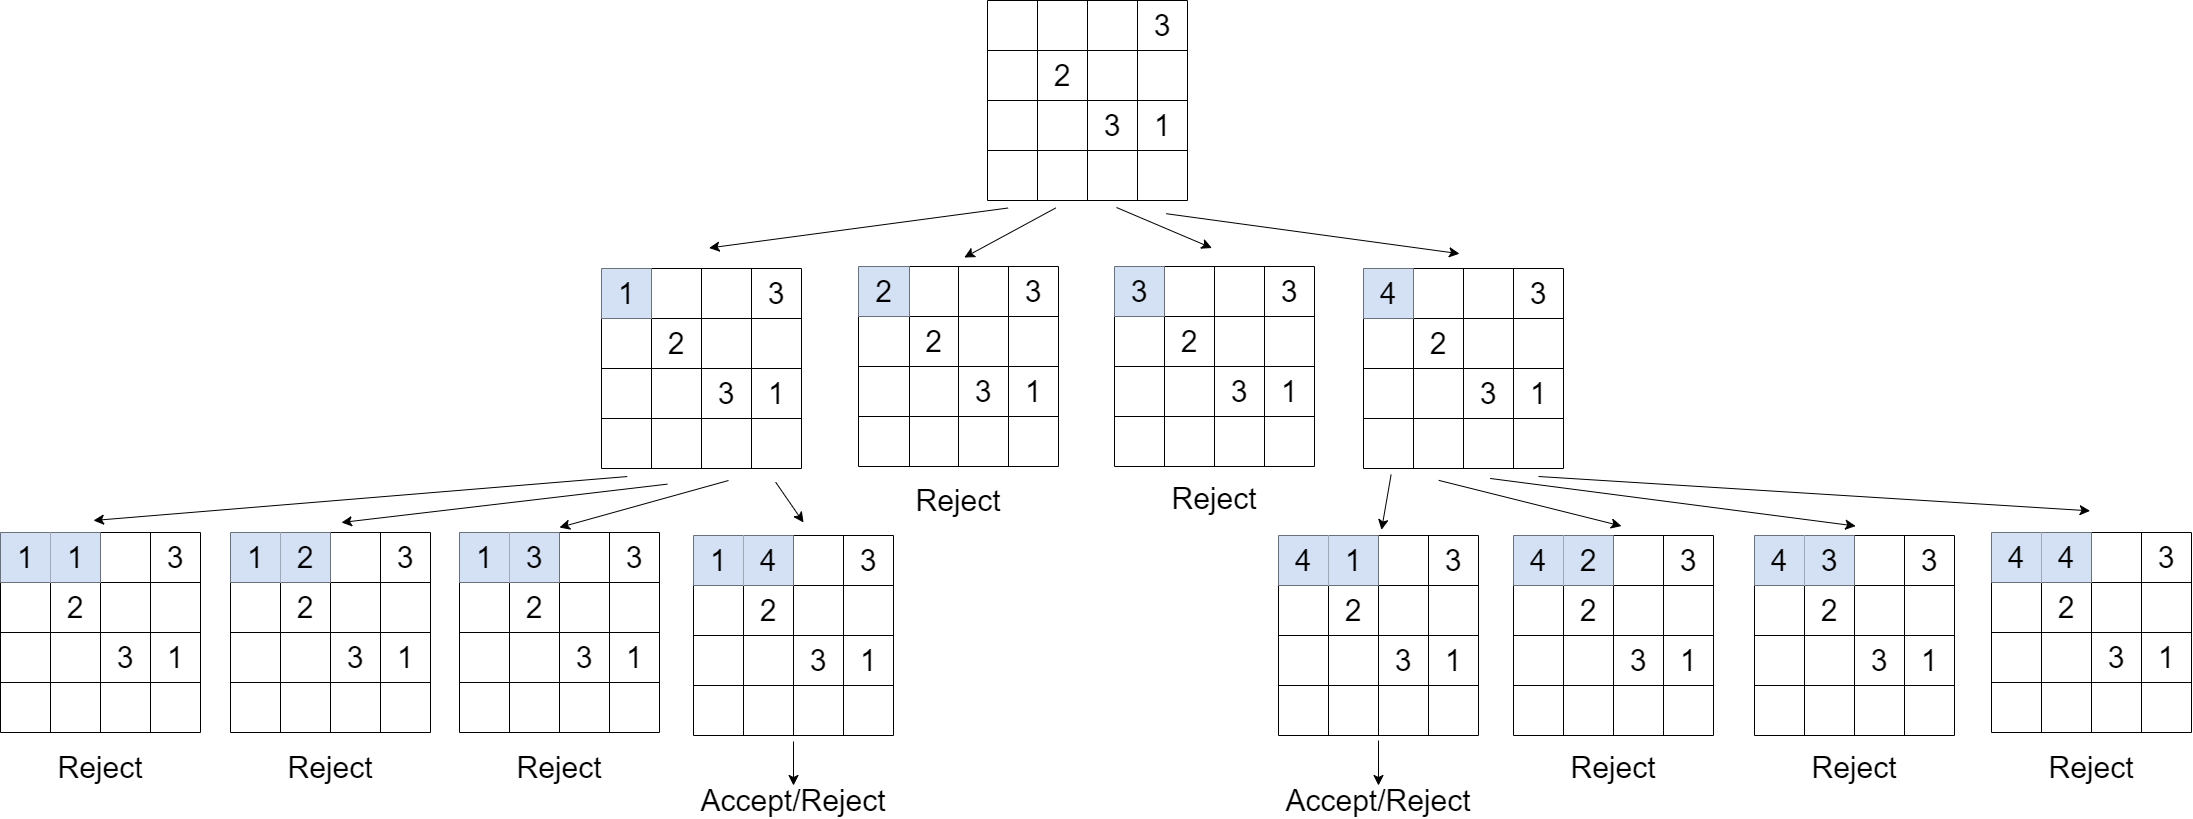
\includegraphics[width=180mm]{figures/turing_non_determinism.png}
	\end{center}
	\caption{\label{ndtm} Non Deterministic Turing Machine with Brute Force Solving}
\end{figure}

\begin{figure}[h!]
	\begin{center}
		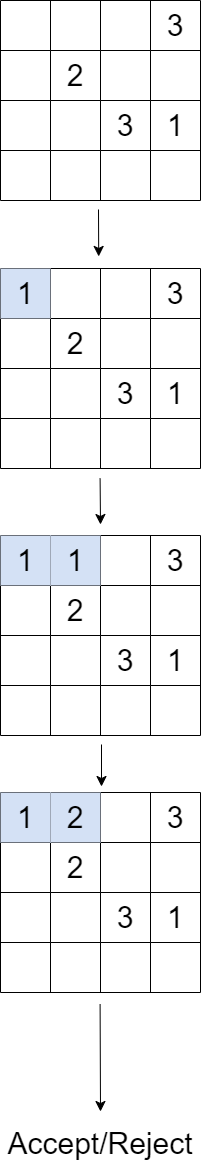
\includegraphics[width=18mm]{figures/turing_determinism.png}
	\end{center}
	\caption{\label{dtm} Deterministic Turing Machine with Brute Force Solving}
\end{figure}

\subsection{Big O Notation}

\textbf{Def$^\text{n}$:} Let $f$ be a function indicating the execution time for an algorithm and $g$ a strictly positive function. $f(x)=O (g(x))$ if $\exists$ positive $ M$ and $x_0$ such that $|f(x)|\leq Mg(x)$ $\forall$ $x\geq x_0$. This is coined \textbf{Big O Notation}.

\textbf{Properties:} Following from the definition we get some immediate properties, assume $f,g,h,i$ are functions obeying the necessary conditions of the definition.
\begin{itemize}
\item Product - $f=O(g)$ and $h=O(i)$, $fh=O(gi)$.
\item Sum - for $f=O(g)$ and $h=O(i)$, $f+h = O(max(g,i))$.
\item Constant Multiplication - for constant $k\neq0$, $O(kg)=O(g)$.
\end{itemize}

\textbf{Def$^n$:} A polynomial time algorithm is an algorithm with $O(x^c)$.

\textbf{Def$^\text{n}$:} A \textbf{Reduction}, $A \leq_p B$, is a transformation in polynomial time ($O(x^c)$) from problem $A$ to $B$.

\begin{figure}[h!]
	\begin{center}
		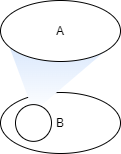
\includegraphics[width=30mm]{figures/reduction.png}
	\end{center}
	\caption{\label{fig:reduction}A$\leq_p$B}
\end{figure}

\subsection{Sets of Difficulty} 

We care about decision problems, these are problems that given an input produce a 'yes' or 'no' answer. We will discuss three sets of these problems:
\begin{itemize}
\item{P (Polynomial) is the the class of problems that can be solved in polynomial time by a deterministic Turing machine;}
\item{NP (Non-deterministic Polynomial) is the class of problems that can be verified in polynomial time by a deterministic Turing machine or solved in polynomial time by a non-deterministic Turing machine;}
\item{the NP-hard class are at least as hard as the hardest NP problem;} 
\item{the NP-complete set is the intersection of NP and NP-hard problems, these are the hardest problems in NP;} 
\item{the coNP class if the complement of all NP problems, for each problem in NP there exists a problem in coNP bu the True and False instances are reversed.}
\end{itemize}

Problems in P are considered feasible and those in NP-complete are infeasible as their complexity scales exponentially with respect to the input size and as it is assumed they cannot be solved in polynomial time ($P \neq NP$) and are therefore infeesible for large inputs. \footnote{We can only assume that $P\neq NP$ as this problem is yet to be proven, it is in fact one of the Millennium Prize problems.}

So when we state sudoku is hard we are actually saying sudoku belongs to NP-complete. We cannot just prove sudoku belongs to NP as this also includes problems in P. \footnote{Due to Ladner's Theorem there exists problem $\in$ NP but $\not\in$ NP-complete and $\not\in$ P iff $P\neq NP$, these problems are called NP-intermediate.}

\begin{figure}[h!]
	\begin{center}
		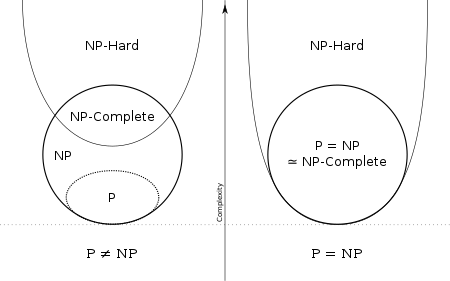
\includegraphics[width=60mm]{P_np.svg}
	\end{center}
	\caption{P, NP, NP-complete \& NP-hard sets\textbf{REDO IMAGE}}
\end{figure}

\subsection{Proving NP completeness?}

Call the problem we wish to prove is NP-complete $x$.

The set of NP-complete problems are defined as members of both the set of NP problems and the set of NP-hard problems. 

First show there exists a verifier for $x$ with a polynomial or less runtime, this is a algorithm that decides if a proposed solution to problem $x$ is correct. This proves $x\in$ NP.

Then take a known NP-complete problem call this $y$, and reduce it to $x$, one does this by transforming the input of $y$ to the input of $x$ in polynomial time, we call this function $g: y\rightarrow x$. Assume there exists a polynomial time algorithm to solve $x$, $f$, then we could solve $y$ in polynomial time too, $f(g(y))$. Therefore if the reduction exists then $x$ is at least as hard as $y$ and as $y$ is NP-complete then $x$ is at least as hard as the hardest question in NP meaning $x \in$ NP-hard.

Therefore $x\in $ NP-complete.

\subsection{The First NP-complete Problem} 

If, as the above suggests, we require a NP-complete problem to prove a problem is NP-complete then we seem to have reached a paradox. Luckily we have the Cook-Levin Theorem.

\textbf{Cook-Levin Theorem:} SAT is NP-Complete. \cite{compcomplexityamodernapproach}

\textbf{Terminology}:
\begin{itemize}
\item Boolean Variable: a variable that can can be true or false ($a=T$ or $a=F$).
\item Literal: a boolean variable or it's negation (if $a = T$ then its negation $\neg a = F$).
\item $\land$: an operation that outputs true when all operands are true, false otherwise ($a\land b = T$ iff $a=T$ and $b=T$).
\item $\lor$: an operation that outputs true when at least one operand is true, false otherwise ($a\lor b = T$ iff $a=T$ or $b=T$).
\item Clause: multiple literals operated on by $\lor$s, a set of clauses are joined by $\land$s.
\item Truth Assignment : assignment of true and false values to each boolean variable. 
\end{itemize}

\textbf{Def$^n$}: SAT is the following decision problem. Given a set of boolean variables $B$ and a collection of clauses $C$ does a valid truth assignment exist that satisfies all clauses in $C$?

Given $B = \{a,b,c\}$ and  $C=\{(a\lor b \lor c \lor \neg c), (a \lor c), (\neg a\lor b)\}$ a valid truth assignments exists. See the table \ref{satex} for all valid assignments.

\begin{table}
\begin{center}
\begin{tabular}{ |c|c|c|c|c|c|c|  }
 \hline
 \multicolumn{7}{|c|}{$(a\lor b \lor c \lor \neg c)\land (a \lor c) \land (\neg a\lor b)$} \\
 \hline
$a$ & $b$ & $c$ & $(a\lor b \lor c \lor \neg c)$ & $(a \lor c)$ & $(\neg a\lor b)$ & Full Clause\\
 \hline
 F & F & F & T & F & T & F \\
\rowcolor{lightgray}
 F & F & T & T & T & T & T \\
 F & T & F & T & F & T & F \\
\rowcolor{lightgray}
 F & T & T & T & T & T & T \\
 T & F & F & T & T & F & F \\
 T & F & T & T & T & F & F \\
\rowcolor{lightgray}
 T & T & F & T & T & T & T \\
\rowcolor{lightgray}
 T & T & T & T & T & T & T \\
 \hline
\end{tabular}
\end{center}
\caption{\label{satex}An example of a SAT clause set with all possible truth assignments explored and valid assignments highlighted.}
\end{table}

We now have a NP-complete problem to reduce other problems to.

\subsection{Examples}

Let's start putting complexity into the context of sudoku. Our input is a grid of size $n\times n$ ($n=D^2$), we will investigate an algorithms run time in comparison to this variable.

\textbf{Constant time, $O(1)$:} This includes functions that take the same time no matter the input size, for example accessing the value of a cell in the sudoku grid, even as the grid increases in size, grid(x,y) takes constant time.

\textbf{Linear time, $O(n)$:} Consider a function that when given a grid and a grid coordinate $(x,y)$ outputs a boolean value; true if the value of the grid at this coordinate is valid (does not repeat in the row, column or box) and false otherwise. Let's consider the inner workings of the function: 
\begin{itemize}
\item First we assume the comparison between two values takes a single unit of time $O(1)$
\item We must compare the value at the given coordinate with each value on the row, observe this is performed $n-1$ times and therefore this operation takes $O(n)$ time.
\item We then compare the value at the given coordinate with each value on the column, as per the previous argument this has complexity $O(n)$.
\item Finally we compare the value with the remainder of the box value that have not been compared previously, this takes $n-(\sqrt{n}-1)-(\sqrt{n}-1)-1= n-2\sqrt{n}+1$ comparison operations which has a complexity of $O(n)$.
\end{itemize}
Overall this function takes $(n-1)+(n-1)+(n-2\sqrt{n}+1) = 3n -2\sqrt{n}-1$ comparisons and therefore calculates the boolean variable in linear time ($O(n)$). See algorithm \ref{alg:validentry}.

\begin{algorithm}
\caption{Validate an Entry}\label{alg:validentry}
\begin{algorithmic}
\Procedure{ValidateEntry}{grid, (x,y), n}
	\For{i = 1 to n} \Comment{Check column}
		\If{i $\neq$ x}
			\If{grid(i,y) = grid(x,y)}
				\State{return False}
			\EndIf
		\EndIf
	\EndFor
	\For{i = 1 to n} \Comment{Check row}
		\If{i $\neq$ y}
			\If{grid(x,i) = grid(x,y)}
				\State{return False}
			\EndIf
		\EndIf
	\EndFor
	\For {i = 1 to $\sqrt{n}$} \Comment{Check box}
		\For {j = 1 to $\sqrt{n}$}
			\If {x DIV $\sqrt{n}$ + i = x and y DIV $\sqrt{n}$ + j = y} 
				\If{grid(x DIV $\sqrt{n}$ + i, y DIV $\sqrt{n}$ + j) = grid(x,y)}
					\State{return False}
				\EndIf
			\EndIf
		\EndFor \Comment{DIV refers to integer division e.g. 7 DIV 3 = 2}
	\EndFor
	\State{return True}
\EndProcedure
\end{algorithmic}
\end{algorithm}

\textbf{Polynomial time, $O(n^t)$}: Consider a function that when given a partially complete sudoku grid returns true if the grid is valid, otherwise it returns false. Using the linear time algorithm we just described we can repeat this for every value within the grid. See algorithm \ref{alg:valid}.

\begin{algorithm}
\caption{Validate a Grid}\label{alg:valid}
\begin{algorithmic}
\Procedure{Validate}{grid,  n}
	\For{i = 1 to n} \Comment{Loop through all (i,j) pairs to validate all squares of the grid}
		\For{j = 1 to n} 
			\If{ValidateEntry(grid, (i,j), n) = False}
				\State{return False}
			\EndIf
		\EndFor
	\EndFor
	\State{return True}
\EndProcedure
\end{algorithmic}
\end{algorithm}

We call ValidateEntry $n^2$ times so our complexity is $O(n\times n^2) = O(n^3)$ this is polynomial and therefore still considered feesible as $n$ increases. 
 
\textbf{Exponential time, $O(a^n)$}: Consider a brute force algorithm to solve sudoku, all we need to do is cycle through values 1 to n for all squares rejecting those that create an invalid sudoku grid and outputting a valid grid if one is found, otherwise false if the sudoku cannot be solved. See algorithm \ref{alg:bruteforce}.

\begin{algorithm}
\caption{Brute Force Sudoku Solver} \label{alg:bruteforce}
\begin{algorithmic}
\Procedure{BruteForceSolve}{grid, n}
	\If{grid is complete}
		\If{Validate(grid) = True}
			\State{return grid}
		\Else
			\State{return False}
		\EndIf
	\EndIf
	\State{(x,y) = location of first empty cell in grid}
	\For{i = 1 to n}
		\State{grid(x,y) = i}
		\If{BruteForceSolve(grid, n) $\neq$ False}
			\State{return grid}
		\EndIf
	\EndFor
	\State{return False}
\EndProcedure
\end{algorithmic}
\end{algorithm}

This algorithm refers to itself, this is called recursion and shall be explored further in chapter 4 when we discussion solving techiques. For now let us see explore this specific algorithm; 
\begin{itemize}
\item Assume we only have 1 empty square then we try the values 1 to $n$ and for each we check if the grid is valid, this takes $O(n\times n^3)$.
\item Now assume we have 2 empty squares we try 1 to $n$ and for every option we have to do the same as the first bullet point which takes $O(n\times n \times n^3)$.
\item A pattern forms, for every empty square we must times the complexity by $n$, we have at most $n^2$ empty squares so the upper bound is $O(n^{n^2+3})$.
\end{itemize}
This algorithm has a complexity that is a bit above exponential as the base is dependent on $n$ too however it is not quite factorial complexity so we will call it exponential. This is infeasible for large values of $n$ and does not belong to P. So solving sudoku is hard, case closed - not quit, this is only one example   of a sudoku solver there may exist more efficient algorithms so we need to disprove this. \footnote{BogoSort is a sorting algorithm that randomises a list until it is in the correct order, this has an unbounded run time, but there exists sorting algorithms with complexity $O(n\text{log}n)$. \textbf{CITE}} 

%%%%%%%%%%%%%%%%%%%%%%%%%%%%%%%



\section{Existance is Hard}
		
Checking if a solution to sudoku exists is NP-complete, let us define the decision problem:

		\begin{equation}
		        \Phi (S) = \begin{cases}
		            \text{True if a completion exists} \\
		            \text{False if a completion does not exist}.
				\end{cases}
		\end{equation}

Our question is does there exist a function $\Phi$ that when given an instance of the problem will, in polynomial time or less,
return True if it can be solved and False otherwise.

\subsection{Proof Outline}

The verifier must be shown to be $\in$ P, this means the Sudoku decision problem belongs to the set NP.

Then we need a reduction from sudoku to a known NP-complete problem to prove sudoku is also NP-hard. We will be creating a chain of reductions: \textbf{Sudoku $\geq_p$ Latin Square $\geq_p$ Triangulated Tripartite $\geq_p$ 3SAT $\geq_p$ SAT}.

\begin{figure}[h!]
	\begin{center}
		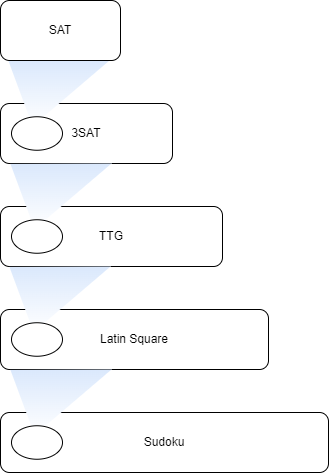
\includegraphics[width=50mm]{figures/subset.png}
	\end{center}
	\caption{\label{fig:sudokureduction}}
\end{figure}

As the Sudoku decision problem is a member of NP and NP-hard it is NP-complete by definition.

\textbf{Note}: Theoretically any problem in the set NP-complete can be reduced to Sudoku and therefore this reduction is not unique, however, it is the most intuitive way. Some readers may question why we are not looking at a reduction to a Graph
$n^2$-Colouring problem but in section \textbf{cite} we explore this is the wrong direction of reduction.

%%%%%%%%%%%%%%%%%%%%%%%
\subsection{Verification is Easy}

Given a sudoku grid $S$, we have an algorithm to determine:
		\begin{equation}
			\Psi(S) = \begin{cases}	
				\text{True if the puzzle is complete} \\
				\text{False if the puzzle is not complete}.
			\end{cases}
		\end{equation}
This algorithm is an extension of algorithm \ref{alg:valid} from the complexity examples, we simply add a for loop to the end to check that $\forall S(i,j) \neq 0 $, in other words there are no empty cells. To find the complexity algorithm we add $n^2$ to the complexity of the original validation algorithm, giving $O(n^2+n^3)=O(n^3)$. This is polynomial time, therefore $\Psi\in $P.
%%%%%%%%%%%%%%%%%%%%%%%
\subsection{Sudoku $\geq_p$ Latin Square}

\textbf{Def$^n$}: A valid Latin Square puzzle is a function $L:i,j \rightarrow x$ for values $i,j \in \{1,..,D\} $ and $x \in
\{0,...,D\}$ satisfying the following:
\begin{itemize}
\item{for all $a,b,c \in \{1,...,D\}$ with $L(a,b) \neq 0 $ and $L(a,c) \neq 0$ then $L(a,b) \neq L(a,c)$}
\item{for all $a,b,c \in \{1,...,D\}$ with $L(a,b) \neq 0 $ and $L(c,b) \neq 0$ then $L(a,b) \neq L(c,b)$}
\end{itemize}
It is complete or solved if for all $i,j \in \{1,...,D\}$, $L(i,j) \neq 0$.

By observation we see this is a superset of the sudoku puzzle, we just add the restrictions that the dimension must be a square number and also add the third property of the sudoku puzzle defintion.

\textit{What is the Latin Square decision problem?} Given a latin square puzzle $L(,)$, can the function be augmented, by changing only the value of the function for value pairs $i,j$ that previously gave $L(i,j) =0$, to get a complete latin square puzzle?

\noindent\rule{4cm}{0.4pt}

\textit{Proof idea:} We must reduce a given latin square grid of size $D \times D$ to a sudoku grid size $D^2 \times D^2$ that is solvable iff the Latin square is.

\textbf{Lemma:} From \cite{sls}: let $S_l$ be a Sudoku problem with the following construction 
\begin{equation}
	S_l(i,j) =\begin{cases}
0 \qquad\qquad\qquad\qquad\qquad\qquad\text{when } (i,j) \in L_s \\ 
((i-1 \text{ mod } n)n + \left\lfloor{i-1/n}\right\rfloor+j-1)\text{ mod } n^2 +1 \quad\text{otherwise}
\end{cases}
\end{equation}
where $L_s=\{(i,j)| \left\lfloor{i-1/n}\right\rfloor=0 \text{ and }(j \text{ mod }n)=1\}$. Then there exists an augmentation $S_l'$ to complete the sudoku puzzle if and only if the square $L$ such that $L(i,j/n)=S_l'(i,j)-1/n+1$ for all $(i,j) \in L_s$ is a Latin square.

\textbf{Note:} The fact we have a formula to generate a valid sudoku for any size $D^2$ is interesting and we should explore if this can be done for a $M\times N$ sudoku too. (explored in section 3). Figure \ref{formula} gives examples of generated sudokus from this formula.

\begin{figure}[h]
\centering
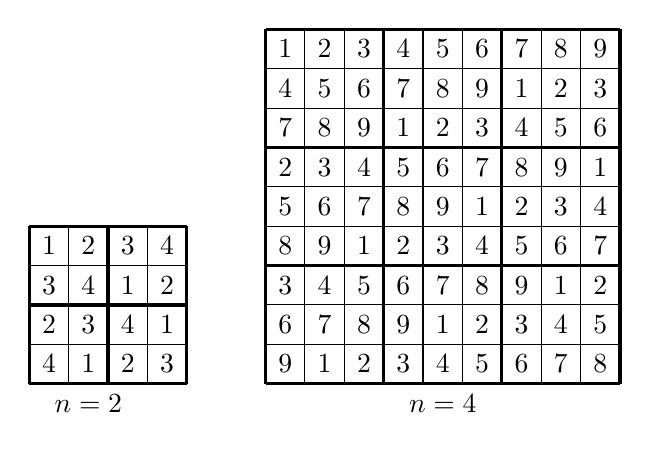
\begin{tikzpicture}[scale=.5]
\begin{scope}[xshift=10cm]
    \draw (0, 0) grid (4, 4);
    \draw[very thick, scale=2] (0, 0) grid (2, 2);
    \setcounter{rowa}{1}
    \setrowa {1}{2}{3}{4}
    \setrowa {3}{4}{1}{2}
    \setrowa {2}{3}{4}{1}
    \setrowa {4}{1}{2}{3} 
    \node[anchor=center] at (1.5, -0.5) {$n=2$};
  \end{scope}
  \begin{scope}[xshift=16cm]
    \draw (0, 0) grid (9, 9);
    \draw[very thick, scale=3] (0, 0) grid (3, 3);
    \setcounter{row}{1}
    \setrow {1}{2}{3}  {4}{5}{6}  {7}{8}{9}
    \setrow {4}{5}{6}  {7}{8}{9}  {1}{2}{3}
    \setrow {7}{8}{9}  {1}{2}{3}  {4}{5}{6}
    \setrow {2}{3}{4}  {5}{6}{7}  {8}{9}{1}
    \setrow {5}{6}{7}  {8}{9}{1}  {2}{3}{4}
    \setrow {8}{9}{1}  {2}{3}{4}  {5}{6}{7}
    \setrow {3}{4}{5}  {6}{7}{8}  {9}{1}{2}
    \setrow {6}{7}{8}  {9}{1}{2}  {3}{4}{5}
    \setrow {9}{1}{2}  {3}{4}{5}  {6}{7}{8}
    \node[anchor=center] at (4.5, -0.5) {$n=4$};
  \end{scope}
\end{tikzpicture}
\caption{Formula Generation of Valid Sudoku}
\label{formula}
\end{figure}

\textit{Proof:}

First we must show $S_l(i,j)=((i-1 \text{ mod } n)n + \left\lfloor{i-1/n}\right\rfloor+j-1)\text{ mod } n^2 +1$ forms a complete and valid sudoku puzzle.

When $i=[1,...,n^2]$ then:
\begin{align}
	0&<\left\lfloor{i-1/n}\right\rfloor<n-1\\
	0&<i-1 \text{ mod } n<n-1\\
	0&<(i-1 \text{ mod } n)n + \left\lfloor{i-1/n}\right\rfloor<n^2-n\\
	0&<(i-1 \text{ mod } n)n + \left\lfloor{i-1/n}\right\rfloor+j-1<n^2-1\\
	1&<((i-1 \text{ mod } n)n + \left\lfloor{i-1/n}\right\rfloor+j-1)\text{ mod } n^2 +1<n^2\\
	1&<S_l(i,j)<n^2
\end{align} 
Note $\left\lfloor{i-1/n}\right\rfloor$ gives the row coordinate when indexed at 0 in which the larger box that (i,j) belongs to starts and $i-1 \text{ mod } n$ gives the row within that box when indexed at 0. Therefore $(\left\lfloor{i-1/n}\right\rfloor,i-1 \text{ mod } n)$ will take all value pairs of integers between 0 and $n-1$.

When j is fixed (particular column), assume two cells have the same value, that is $S_l(i,j)=S_l(i',j)$ then
\begin{align}
(i-1 \text{ mod } n)n + \left\lfloor{i-1/n}\right\rfloor+j-1 &= (i'-1 \text{ mod } n)n +
\left\lfloor{i'-1/n}\right\rfloor+j-1\\
	(i-1 \text{ mod } n)n + \left\lfloor{i-1/n}\right\rfloor &= (i'-1 \text{ mod } n)n + \left\lfloor{i'-1/n}\right\rfloor
\end{align}
from the above $i=i'$. No cell on a column has the same value.

When i is fixed (particular column) assume two cells have the same value, that is $S_l(i,j)=S_l(i,j')$ implies $j-1=j'-1 (\text{mod }n)$ therefore $j=j'$.

For the third condition fix $\left\lfloor{i-1/n}\right\rfloor$. (i-1 \text{ mod } n,j) takes all value pairs of integers 0 to n-1 so if a cell has the same value as another within the n by n square $S_l(i,j)=S_l(i',j')$ implying $(i-1 \text{ mod }n,j)=(i'-1 \text{ mod } n,j')$ which means $i=i'$ and $j=j'$. Therefore $S_l$ is a valid and complete sudoku puzzle.

Now consider which integers fill the blanks in $L_s$. For $(i,j)\in L_s$, $S_l(i,j)-1= ((i-1 \text{ mod } n)n+j-1)\text{ mod } n^2$ as $j mod n=1$, $j-1modn=0$ therfore $S_l(i,j)-1$ is divisible by n so $S_l-1/n+1$ gives integers between $[1,...,n]$.
Therefore $L(i,j) \in [0,...,n]$.

We must validate the Latin square conditions. The row constraint in $S_l$ ensures $S'(i,j)=S'(i,j') \implies j=j'$, $S'(i,j)-1/n+1=S'(i,j')-1/n+1 \implies j=j'$, $L(i,j/n)=S'(i,j'/n) \implies j=j'$ is equivalent to the row constraint of L. The column constraint of $S_l$ is equivalent to the column constraint of L. The small square constraint of $S_l$ is equivalent to the column constraint of L. $\square$

\subsection{Latin Square $\geq_p$ Triangulate A Tripartite Graph}

\textbf{Def$^n$}: A graph $G=(V,E)$ is tripartite if a partition $V_1$, $V_2$, $V_3$ exists such that the vertices are split into three sets with no edges between vertices that belong to the same set, i.e for all $(v_i,v_j) \in E\text{ if } v_i \in V_i\text{ then }v_j \not\in V_i $.

\textbf{Def$^n$:} A triangulation T of a graph is a way to divide edges into disjoint subsets $T_i$, each forming a triangle ($T_i=\{(v_{1}, v_{2}),(v_{2}, v_{3}),(v_{3},v_{1})\}$).

If a tripartite graph can be triangulated it must be uniform, that is: every vertex in $V_1$ (or $V_2$ or $V_3$) has the same number of neighbour in $V_2$ and $V_3$ (or the respective sets).

\textit{What is the Triangulated Tripartite decision problem?} Given a graph G that is tripartite (can be split into 3 subgroup, within these subgroups vertices should not share edges) can it be triangulated?

\noindent\rule{4cm}{0.4pt}

\textbf{Theorem:} From \cite{lsttg}: completing a Latin square with dimensions n by n is equivalent to triangulating a tripartite graph $G= V_1, V_2, V_3$.

\textit{Proof:} 

Intuitively, we map a graph to a Latin square $L$ through the following: 
given tripartite graph G=(V,E) label vertices in $V_1$ with distinct lables $\{r_1,...r_n\}$, label vertices in $V_2$ with distinct lables $\{c_1,...c_n\}$ and label vertices in $V_3$ with distinct lables $\{e_1,...e_n\}$. Add edges such that:
\begin{itemize}
\item{If $L(i,j) = 0$ then add the edge $(r_i,c_j)$ }
\item{If for all $i \in [0,...,n]$ and constant j, $L(i,j) \neq k$ then add the edge $(r_i,e_k)$}
\item{If for all $j \in [0,...,n]$ and constant i, $L(i,j) \neq k$ then add the edge $(c_j,e_k)$}
\end{itemize}
This graph has a triangulation iff $L(i,j)$ can be solved.

Let us show every uniform tripartite graph can be transformed to the above formulation of a Latin square.

\begin{figure}[h!]
\centering
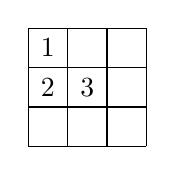
\begin{tikzpicture}[scale=.5]
\begin{scope}[xshift=10cm]
    \draw (0, 0) grid (3, 3);
    \setcounter{rowb}{1}
    \setrowb {1}{}{}
    \setrowb {2}{3}{}
    \setrowb {}{}{}
  \end{scope}
\end{tikzpicture}

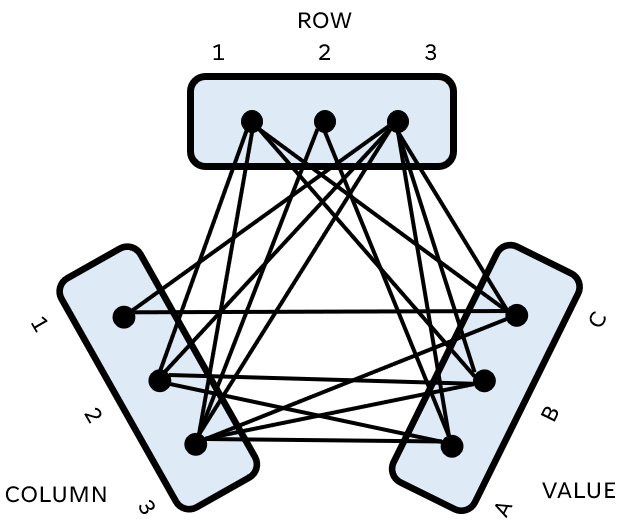
\includegraphics[height=40mm]{figures/ttg.png}
\caption{The Latin Square is equivalent to the Tripartite Graph.}
\end{figure}

First we need a generalisation of a latin square

\textbf{Def$^n$}: A Latin framework LF for tripartite graph G, size (r,s,t) is a r by s array with values [1,...,t]. With constraints:
\begin{itemize}
\item{Each row/column contain each element only once.}
\item{If $(r_i,c_j)\in E$ then LF(i,j)=0 else LF(i,j)= k, $k\in [1,...,t]$}
\item{If $(r_i,e_k)\in E$  then $\forall j$ $LF(i,j)\neq k$}
\item{If $(c_j,e_k)\in E$  then $\forall i$ $LF(i,j)\neq k$}
\end{itemize}
If r=s=t then LF is a latin square (formulation above) which can be completed iff G has a triangle partition.

\textbf{Lemma}: For tripartite graph G=(V,E) with $|V_1|=|V_2|=|V_3|=n$ (uniform), there's a Latin framework of (n,n,2n).

\textit{Define LF an n by n array. For $(r_i,c_j)\in E$ $LF(i,j)=0$ else $LF(i,j)=1+n+((i+j)\text{ mod }n)$. LF is a latin framework as the first two bullet points of the definition hold by construction and as $1+n\leq LF(i,j)\leq 2n$ LF will never equal a value in $1,...n$ and therefore the last two bullet points hold. The size is trivial. $\square$}

\textbf{Lemma}: Given latin framework LF(n,n,2n) for uniform tripartite graph G, we can extend the latin framework to have size
(n,2n,2n).

\textit{First we have a few denotions: R(k) = the number of times k appears in L plus half $|e_k|$; $S_i=\{k|k \not\in LF(i,j) \forall j \cap (r_i,e_k)\not\in E\}$; $M=\{k|R(k)=r+s-t\}$. We show sets $S_1,...S_r$ have a system distinct representative (\textbf{DEFINE}) containing all elements of $M$, we then add this system as the $(s+1)$st column and repeat until we have $2n$ columns.}

\textit{Using Hoffman and Kuhn's theorem \cite{hoffman} we need only show that $S_1,...S_r$ have a system distinct representative and that for every $M'\subseteq M$ at least $|M'|$ of sets $S_1,...S_r$ have non empty subsections with $M'$.}

\textit{First choose any $m$ sets such that $1\leq m \leq r$. As G is uniform each set has t-s elements, so $m$ sets together have $m(t-s)$ cardinality. Each value $1,...,t$ appears at least r+s-t times in $LF$, so note each value appears in at most $t-s$ of the sets $S_i$. Consider the union of the $m$ sets, this contains some $p$ elements so we have $p(t-s)\geq m(t-s)$ therfore $p\geq m$. So any $m$ sets have at least $m$ elements in their union and by Hall's theorem \cite{hall} a system distinct representative exists.}

\textit{Next take $M'\subseteq M$ and assume there are $p$ sets in $S_1,...S_r$ that have a nonempty intersection with $M'$. Each set has $t-s$ elements and together have caridinality $p(t-s)$, each element of $M$ appears in exactly $r-(r+s-t)=t-s$ of the $s_i$s, therefore $|M'|(t-s)\leq p(t-s)$ so $|M'|\leq p$. At least $|M'|$ sets have nonempty intersections with $M'$.}

\textit{The Hoffman and Kuhn theorem holds and therefore a system distinct representative exists and can be added to the end. We repeat this n times.} $\square$

\textbf{Lemma}: Latin framework (n,2n,2n) for grpah G, can be extended to (2n,2n,2n).

\textit{We can transpose the array and do the same as the previous lemma. $\square$}

\textbf{Note}: we can find a system distinct representative using the Hopcroft-Karp \cite{hopcroft} algorithm which solves bipartite matching in polynomial time. 

Given a tripartite graph G, if it is not uniform then no triangulation exists, else we apply above to produce a latin framework of size (2n,2n,2n) in polynomial time. This is a Latin square which can be completed iff G has a triangulation. The latin square problem has been reduced to the triangulating a tripartite graph problem. $\square$

\subsection{Triangulated Tripartite $\geq_p$ 3SAT}

\textit{What is 3SAT?} With a set of boolean variables $B$ and a collection of clauses $C$, with at most 3 literals (a literal is any $b \in B$ or its negation $\bar{b}$) in each, does a valid truth assignment exist that satisfies $C$?
		\begin{equation}
		        \phi (C,B) = \begin{cases}
		            \text{True if a truth assignment exists} \\
		            \text{False if a truth assignment does not exist}.
				\end{cases}
		\end{equation}
This decision problem is therefore an enforced limitation of SAT as defined in the section Computational Complexity.

\noindent\rule{4cm}{0.4pt}

\textit{Proof:}

This reduction is a little trickier as we need to introduce the Holyer graph $H$ from \cite{holyer}, this graph has the topology of torus.

\textbf{Def$^n$}: The Holyer graph $H_{3,p}$ is the set of vertices $V=\{(x_1,x_2,x_3)\in \mathbb{Z}_p^3 \| x_1+x_2+x_3 \equiv 0 (mod p)\}$ and an edge exists between vertices $(x_1,x_2,x_3)$ and $(y_1,y_2,y_3)$ if distinct i,j and k exist such that:
\begin{itemize}
\item $x_i\equiv y_i (\text{mod }p)$
\item $x_j\equiv y_j+1 (\text{mod }p)$
\item $x_k\equiv y_k-1 (\text{mod }p)$
\end{itemize}
See figure \ref{holyer} for an example.

\begin{figure}[h!]
\begin{center}
		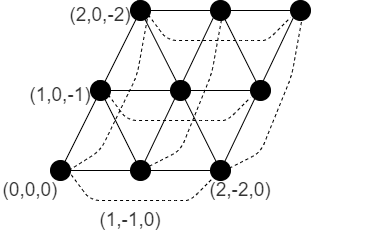
\includegraphics[height=40mm]{figures/holyer_coord.png}
		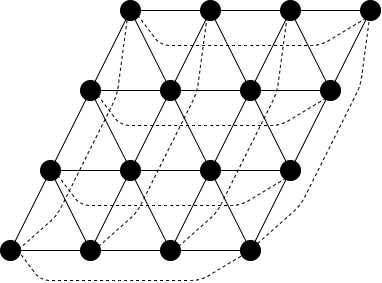
\includegraphics[height=40mm]{figures/holyer_3_4.png}
\end{center}
		\caption{$H_{3,2} $ and $H_{3,3}$, the torus is embedded in the 2 dimensional plane, dotted lines link vertices that are the "same".}
		\label{holyer}
\end{figure}

This graph is tripartite if and only if $p\equiv 0 $ (mod 3), this is demonstrated by a 3-colouring (a graph is tripartite if and only if it is 3-colourable) in figure \ref{holyercolour}.

\begin{figure}[h!]
\begin{center}
		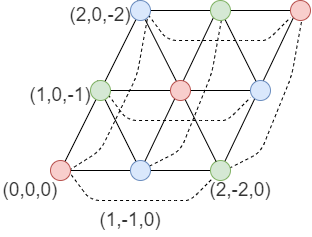
\includegraphics[height=40mm]{figures/colour_holyer_coord.png}
		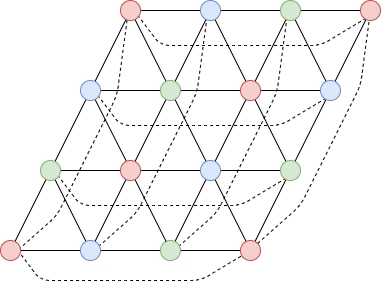
\includegraphics[height=40mm]{figures/colour_holyer.png}
\end{center}
		\caption{3-colouring of $H_{3,2} $ and $H_{3,3}$ }
		\label{holyercolour}
\end{figure}

\textbf{Def$^n$}: $H_{3,p}$ has only two triangulations, termed a true and a false triangulation, see figure \ref{truefalsetri}. 

\begin{figure}[h!]
\begin{center}
		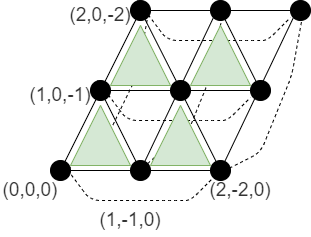
\includegraphics[height=40mm]{figures/holyer_true_triangulation.png}
		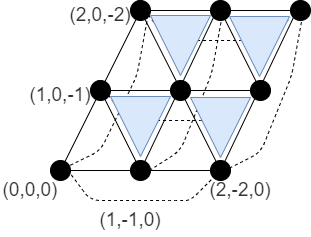
\includegraphics[height=40mm]{figures/holyer_false_triangulation.png}
\end{center}
		\caption{True triangulation and a False triangulation on a $H_{3,2}$ graph. Notice the edges between (0,0,0), (1,0,-1) and (1,-1,0) uniquely determine the triangulation; if they belong to the same triangle then it is a true triangulation and false otherwise.}
		\label{truefalsetri}
\end{figure}

\textbf{Note:} We connect graphs together by taking a set of vertices in $G_1$ and making them the 'same' as a set of vertices in $G_2$, sets are the same size.

\textbf{Def$^n$}: We will connect out graph with F-patches and T-patches, see figure \ref{patches}. 

\begin{figure}[h!]
\begin{center}
		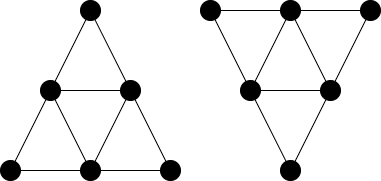
\includegraphics[width=70mm]{figures/patches.png}
\end{center}
		\caption{F-patch and a T-patch}
		\label{patches}
\end{figure}

Let's turn an instance of 3SAT into an instance of triangulating a tripartite graph through the following transformation process: (select p large enough to prevent patch overlap and  $p\equiv 0 $ (mod 3))
\begin{itemize}
\item For $b_i\in B$ create $H_{3,p}$ called $G_{b_i}$.
\item For all $c_j\in C$, for each literal $l_{i,j}$ $j\in [1,2,3]$ create $H_{3,p}$ called $G_{i,j}$.
\item If $l_{i,j}=b_k$ connect an F-patch in $G_{b_k}$ to an F-patch in $G_{i,j}$, else if $l_{i,j}=\neg b_i$ connect a F-patch in $G_{i,j}$ to a T-patch in $G_{b_k}$.
\item For each $i$ connect one F-patch from each $G_{i,1}$, $G_{i,2}$ and $G_{i,3}$ then delete the centre triangle. 
\item $G = \{G_{b_i}$ $|$ $b_i \in B\}\cup\{G_{i,j}$ $|$ $ c_j\in C\text{ and }i\in [1,..,3] \}$
\end{itemize}
We now need to prove the graph produced by this transformation can be triangulated if and only if there is a truth assignment satisfying the 3SAT formula.

Assume a triangulation of G exists, consider a H within the construction of G. H is eitehr a true triangulation or a false triangulation. Now assume $l_{i,j}$ is $b_k$ and consider the join between $G_{i,j}$ and $G_{b_k}$ as this joins two F-patches we get at least one true triangulation: if $G_{i,j}$ is a true triangulation this acounts for all edges near the joining patch but the actual patch can be attributed to $G_{b_k}$ which can be triangulated either way; if both are false triangulations the connecting patch is forced to belong to both $G_{i,j}$ and $G_{b_k}$ which is a contradiction. (Figure \ref{holyerone})

\begin{figure}[h!]
\begin{center}
		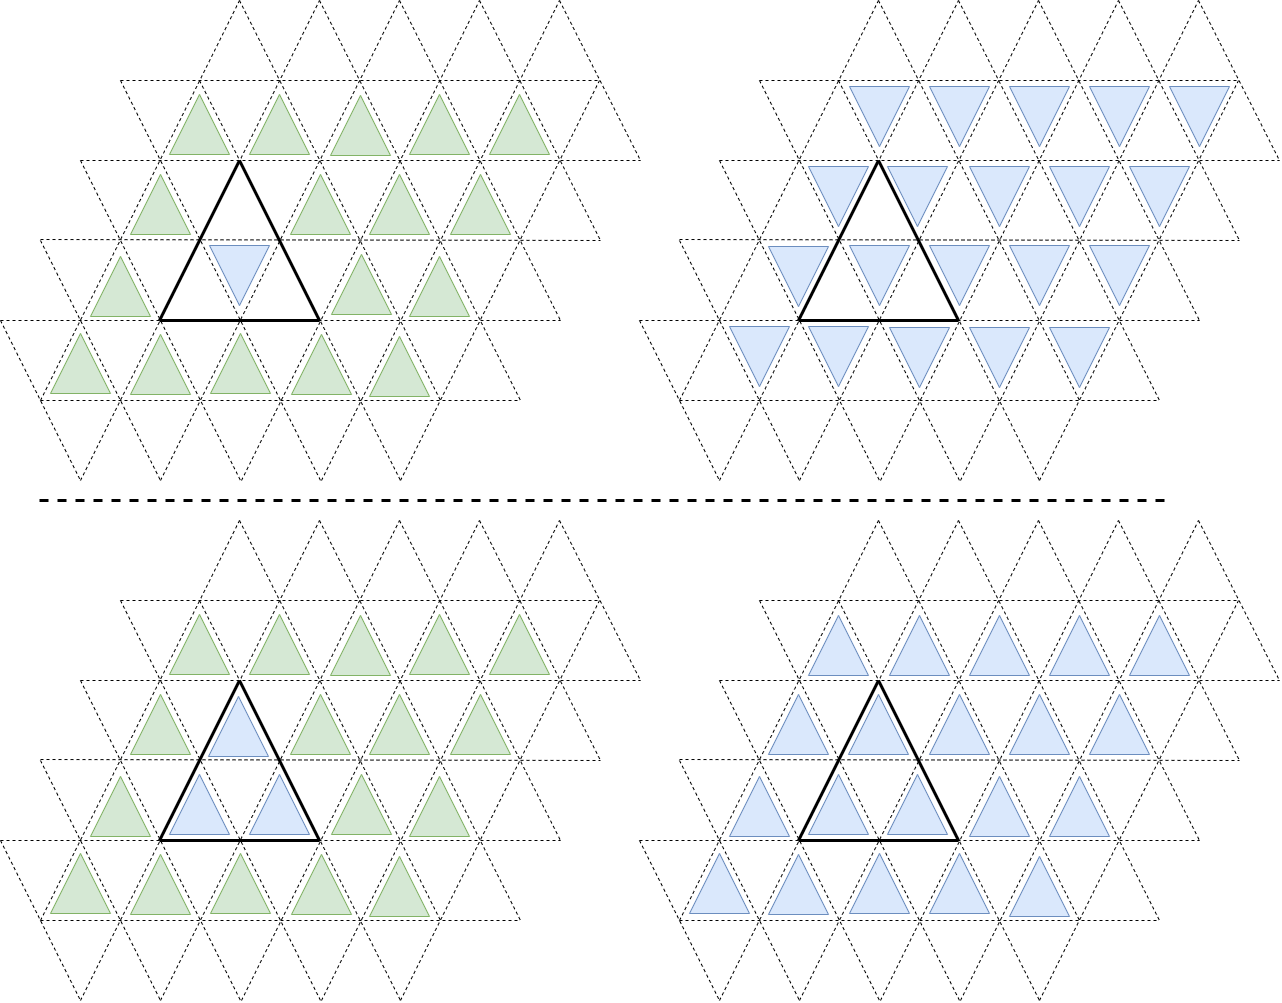
\includegraphics[width=100mm]{figures/first_holyer_lemma.png}
\end{center}
		\caption{Graphs connected by two F-patches, the only complete triangulations are shown, one of each or two true triangulations.}
\label{holyerone}
\end{figure}


Similarly if  $l_{i,j}=\neg b_i$ then $G_{i,j}$ is a false triangulation or $G_{b_k}$ is a true triangulation. (Figure \ref{holyertwo})

\begin{figure}[h!]
\begin{center}
		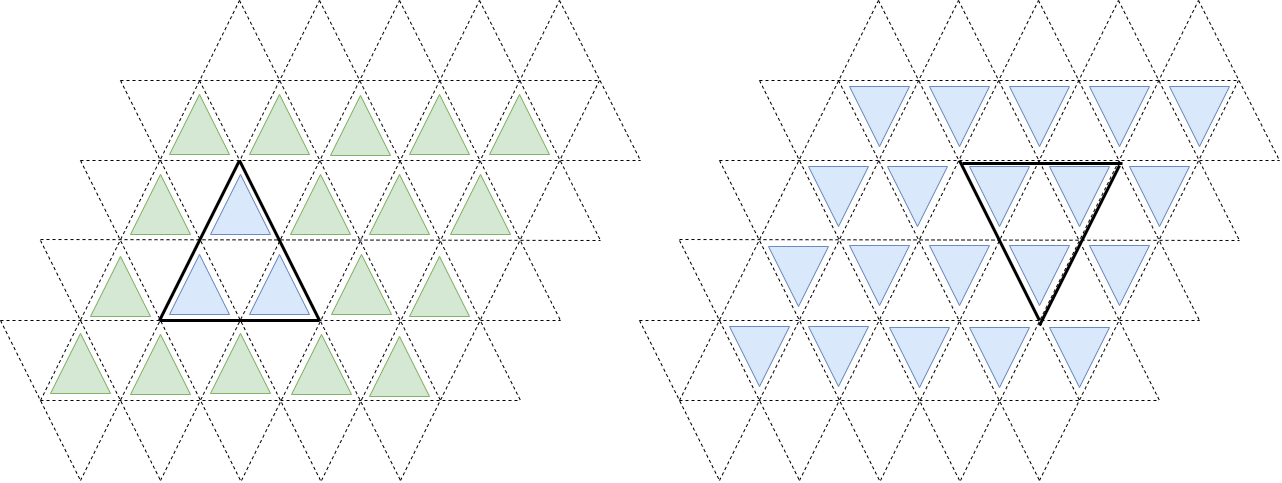
\includegraphics[width=100mm]{figures/lemma_two_holyer.png}
\end{center}
		\caption{Graphs connected by a T-patch and a F-patch, the only complete triangulation is show.}
\label{holyertwo}
\end{figure}

Next the join between clause graphs allow for one false triangulation and the rest  are true triangulations. As the centre of the patch is missing a single $G_{i,j}$ must take the outer edges of the patch by being a false triangulation. (Figure \ref{holyerthree})

\begin{figure}[h!]
\begin{center}
		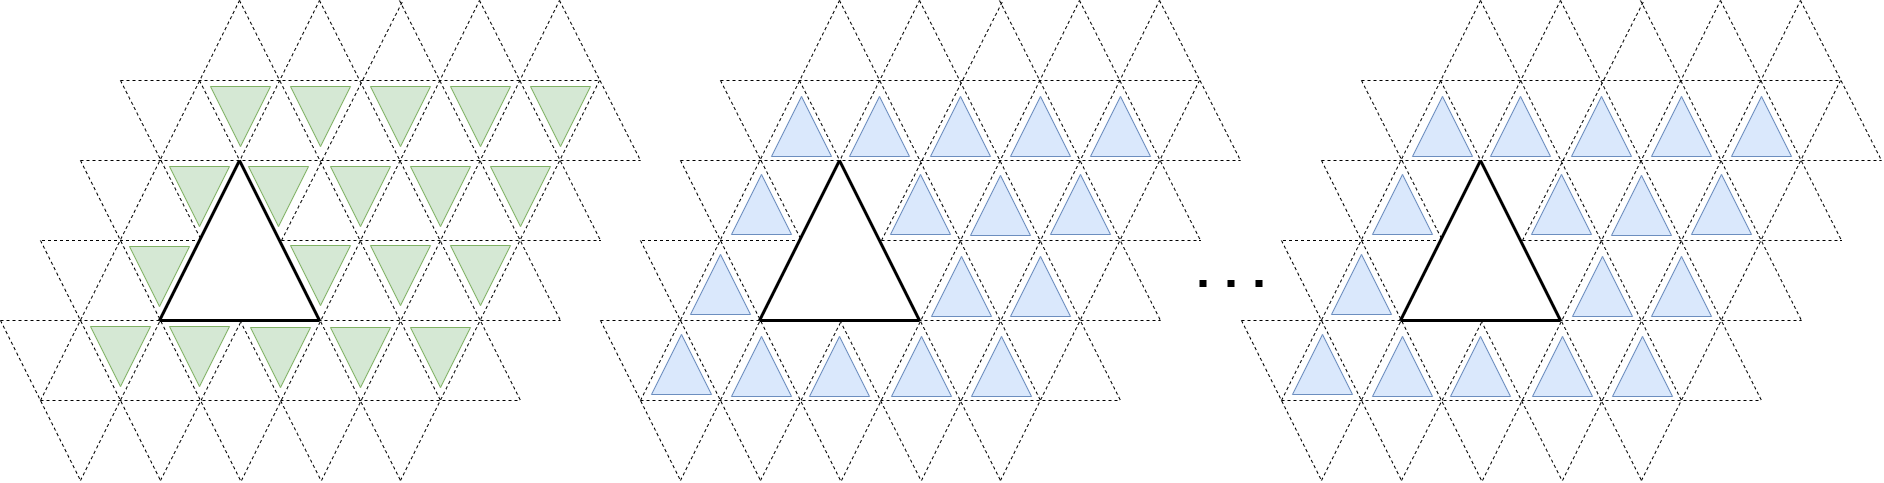
\includegraphics[width=120mm]{figures/lemma_three_holyer.png}
\end{center}
		\caption{Graphs connected by F-patches with the centre removed, the only complete triangulation is show, exactly one must be a false triangualtion.}
\label{holyerthree}
\end{figure}

If G can be triangulated a truth assignment exists such that variable $b_k$ is true if $G_{b_k}$ has a true partition otherwise it is false.

If there exists a truth assignment we can triangulate $G_{b_k}$ according to this truth assignment and this will allow for the whole graph to be triangulated.

This transformation takes place in polynomial time and therefore Triangulated Tripartite $\geq_p$ 3SAT. $\square$

\subsection{3SAT is NP-Complete}
%%%%% define clause

\textit{Proof:}

Given a truth assignment $t$ check each clause is satisfied, if all are satisfied return True else False, this algorithm is at most the length of $C$ multiplied by the length of $B$. $O(BC)$ is polynomial, a polynomial verifier exists.

Given a SAT instance with the input sets of $B$ and $C$. $C$ is in conjunctive normal form (every clause set can be converted to an equivalent set in CNF form ) such that $\forall c \in C$ and for some $b_1, ... ,b_n \in B$, $c = b_1 \lor b_2
\lor ... \lor b_n$. For each $c \in C$ with more than 3 literals we can transform these to a new set of clauses of length 3.

For $c = b_1 \lor b_2 \lor ... \lor b_n$ we introduce a new literal: $a_1$ to give $b_1 \lor b_2 \lor a_1$, $\bar{b_1} \lor a_1$, $\bar{b_2} \lor a_1$ and $a_1 \lor b_3 \lor ... \lor b_n$. Then $a_1 \lor b_3 \lor ... \lor b_n$ becomes $b_3 \lor b_4 \lor a_2$, $\bar{b_3} \lor a_2$, $\bar{b_4} \lor a_2$ and $a_1 \lor a_2 \lor b_5 \lor ... \lor b_n$. This continues at most $n/2$ times to give $a_1 \lor ... \lor a_{n/2}$ or $a_1 \lor ... \lor a_{n/2} \lor b_n$ if n is odd.

Because we can convert a clause larger than 3 into multiple clauses of at most 3 literals in linear time ($O(n/2 + n/4 + ...) = O(n)$) this means we can reduce SAT to 3SAT in polynomial time.

As SAT is NP-complete by the Cook-Levin Theorem, this proves 3SAT is NP-Complete. $\square$
		
\begin{figure}
\begin{center}
		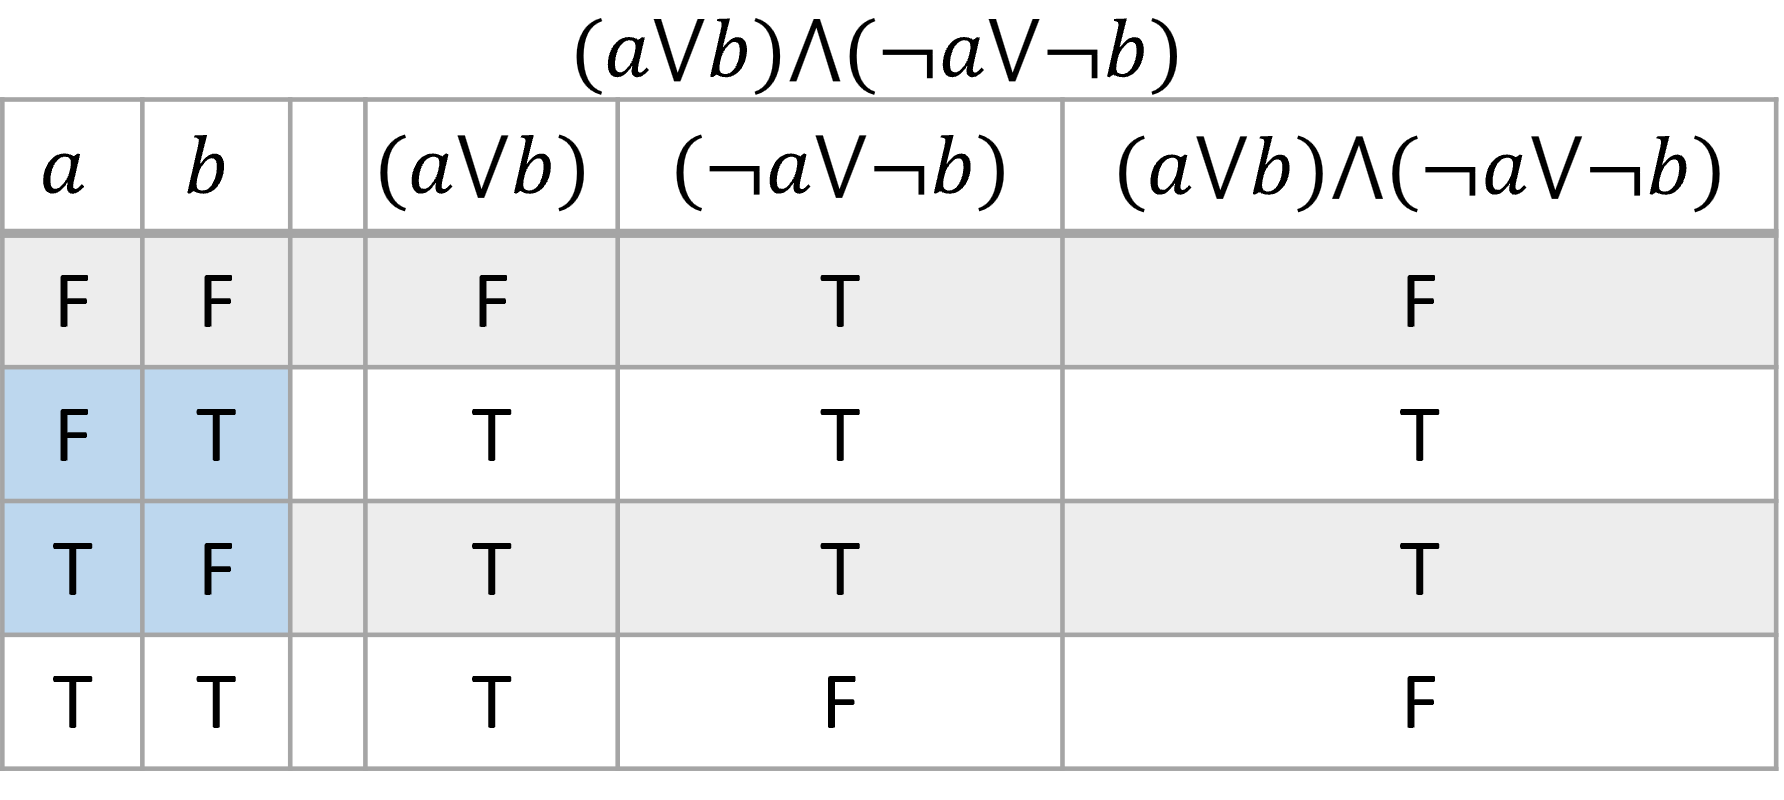
\includegraphics[width=70mm]{figures/sat_example.png}
\end{center}
		\caption{Truth Assignment Example with Highlighted Valid Assignment}
\end{figure}

\noindent\rule{4cm}{0.4pt}

\textbf{Wrap Up} 

$\Phi\in $ NP as $\exists$ a verifier $\Psi$ when given an instance $S$ can determine if it is complete/solved in polynomial time, $\Psi\in$ P.

$\Phi\in $ NP-hard as an instance of SAT can be reduced to an instance of 3SAT in polynomial time which can be reduced to an instance of Triangulating a Tripartite Graph in polynomial time which can be reduced to an instance of Latin Square in polynomial time which can be reduced to an instance of Sudoku ($\Phi$) in polynomial time.

As $\Phi\in$ NP and $\Phi\in$ NP-hard, $\Phi\in$ NP-complete. $\square$

Determining if a sudoku grid $S$ has a completion is suspected hard and infeasible for large $D$.

\subsection{Sudoku $\leq_p$  Graph Colouring}

When reducing sudoku to a grpah problem the obvious thought is to change it to a $D^2$-colouring which we also know to be NP-complete. Unfortunately, this is the incorrect way round, while all sudokus can be turned into a $D^2$-colouring problem it is not immediately obvious how to change all 9 colouring problems into the input of the sudoku decision problem. 

To transform a grid $S$ to sudoku:
\begin{itemize}
\item For each cell of the grid we create a vertex; $\forall i,j\in D^2$ create vertex $v_{i,j}$, giving $D^4$ vertices in total.
\item Create edges such that: for each $i$ $(v_{i,j},v{i.k})\in E$; for each $j$ $(v_{i,j},v{k.j})\in E$ and for $\lfloor\frac{i-1}{D}\rfloor\equiv\lfloor\frac{k-1}{D}\rfloor$ and $\lfloor\frac{j-1}{D}\rfloor\equiv\lfloor\frac{l-1}{D}\rfloor$, $(v_{i,j},v_{k,l})\in E$.
\item Then for all $D^2$ colours assign a numerical value and for all $S(i,j)\neq 0$ assign the $v_{i,j}$ the colour associated with value $S(i,j)$.
\end{itemize}

Now all sudoku problems can be converted to a $D^2$- colouring problem in polynomial time and since we have proven sudoku is NP-complete as long as $D^2$- colouring has a polynomial verifier (which is trivial to check) then it is also NP-complete.  

This emphasises the importance of the reduction direction, it is easy to transform a problem in P to a problem in NP in polynomial time (it is easy to make something more complicated than it needs to be) but the other way round has not yet been done. 

\subsection{Dimension Analysis}

The large string of reductions performed to change a SAT instance into a Sudoku instance can shroud the link between the two as the proofs are somewhat flamboyant, let us abstract the proofs away and focus on the change in size of the SAT instance to a Sudoku instance. Note that this is not conclusive as from definition of NP-complete class we know there is multiple ways to create a reduction and one may be more efficent than what we have described, but it is interesting to visit the problem from a view of space complexity (the memory used when computing a result).

A SAT instance with $A$ clauses and $B$ variables is transformed into a 3SAT instance with $A + 3a$ clauses and $B+a$ variables where $a=\Sigma_{c\in C'}|c|-3$, $C'=\{c\in C | |c|>3\}$. \textbf{PROOF BY INDUCTION NEEDED?}

A 3SAT instance with $C$ clauses and $D$ variables is transformed into a Triangulating a Tripartite Graph instance with $p(D+3C)$ nodes where $p\equiv 0 (\text{mod}3)$.

A Triangulating a Tripartite Graph instance with $E$ nodes is transformed into a Latin Square instance with dimension $\frac{2}{3}E$.

A Latin Square instance with dimension $F$ is transformed into a Sudoku with dimension $F^2$.

In summation, a SAT instance of $A$ clauses and $B$ variables becomes a sudoku instance of dimension $(\frac{2}{3}p(3A+B+10a))^2 $.

\textbf{AN EXAMPLE TRANSFORMATION}

\section{Solving Sudoku is Hard}

We have only focused on decision problems with a boolean yes or no answer so far, but, when it comes to being given a sudoku most people assume it is solvable and then search for a solution so let us change our perspective to search problems; is it hard to solve sudoku? 

\begin{equation}
\Gamma(S) =  S' \text{ if $\exists$ a completed $S$ else 0}
\end{equation}
Where $S'$ is a completed version of $S$.

It is intuitive that the search problem is harder than the decision problem but let's quantify this into our concepts of P and NP. If $P \neq NP$ then both are infeesible to solve as the search problem is harder than an NP-complete decision problem. However, we have hope, if $P=NP$ the corresponding search problem to an NP decision problem $\Gamma$ can be solved in polynomial time. 

\textbf{Theorem}: From \cite{compcomplexityamodernapproach}. Suppose $P=NP$ then for every problem $\rho\in$ NP there exists a polynomial time Turing Machine $T$ that on input $x$ where $\rho(x)=True$ will output a certificate of $x$.

\textbf{Note:} A certificate in complexity theory refers to a solution path of the decision problem, here it is a completed sudoku grid that is the augmented version of the input. 

\section{Determining Uniqueness is Hard}

\textbf{Def$^n$:} The Sudoku Uniqueness problem is: Given a partially completed sudoku grid $S$ does there exist exactly 1 completion?
		\begin{equation}
		        \Gamma (S) = \begin{cases}
		            \text{True if only one completion exists} \\
		            \text{False if multiple completions or none exist}.
				\end{cases}
		\end{equation}

This decision problem belongs to the class called Difference Polynomial Time (or DP/ BH$_2$) \cite{dpcomplexity}.

\textbf{Def$^n$:} DP is the class of problems which are the intersection of a problem in NP and a problem in coNP, this is not NP $\cap$ coNP, it is all problems $\Delta$ such that for $a \in $NP and $b\in $coNP:
		\begin{equation}
		        \Delta (x) = \begin{cases}
		            \text{True if $a(x)$ and $b(x)$ are True} \\
		            \text{False otherwise }.
				\end{cases}
		\end{equation}

We can reformulate the definition of $\Gamma$ to immediately show $\Gamma\in$ DP. Instead of saying uniqueness is satisfied by all sudoku grids that have a single solution, we can say it is all sudoku grids that have a solution minus all sudoku grids that have at least two solutions; this is the same as $\Delta = \Phi \cap \bar{\Upsilon}$ when $\Upsilon$ is the problem satisfied by sudokus that have at least two solutions. We know already $\Phi\in$ NP now we must show $\Upsilon$ is in NP which is easily done; when given a sudoku and two or more solutions it is easy to verify these separately (as shown in Verification is Easy).$\bar{\Upsilon}$ is satisfied by sudokus with one or no solution and is in coNP by definition. Therefore the intersection of $\Phi$ and $\bar{\Upsilon}$ gives $\Delta$, this formulation is exactly what is needed for $\Gamma\in$ DP.

This is helpful but now we must determine the difficulty of DP \cite{dphardness}. \textbf{SEE BOOLEAN HIERARCHY WIKI}
		
% ~~~~~~~~~~~~~~~~~~~~~~~~~~~~~~~~~~~~~~~~~~~~~~~~~~~~~~~~~~~~~~~~~~~~~~~~~~~~~~~~~~~~~~~~~~~~ %

\chapter{Solving Techniques}
Chapter 2 showed it is hard to solve sudoku, yet a quick google search will yield many websites that do the exactly that. We take this chapter to explore how we go about designing optimising and ensuring mathematical rigor in our solution algorithms.
\section{Pencil Solutions}
Taking a human approach we shall see if this sheds any light on the problem.

Given an incomplete sudoku puzzle $p\in P_n$ how does one go about completing this.

The easiest technique to observe and implement is coined a Forced cell. Given an empty cell ($p(x,y)=0$) in C$x$ R$y$ B$z$ this cell is forced if the set $F=\{1,...,n\} / \{$ C$x$ $\cup$ R$y$ $\cup$ B$z$ $\}$ has only one element. This is to say $p(x,y)$ has only one valid value other than 0. 

The remining techniques require pencil marks, that is for the average player, notes in each of remaining candidates ($F=\{1,...,n\} / \{$ C$x$ $\cup$ R$y$ $\cup$ B$z$ $\}$), usually only notes if less than 3 or 4 candidates exist. Denote the candidate set for the cell with C$x$ R$y$ B$z$ as $F_{x,y,z}$. $F_{\text{C}x} = \{F_{x,i,j}|i\in\{1,...,n\}, j \in \text{set of boxes C$x$ passes through}\}$, the corresponding definition for $F_{\text{R}x}$ and $F_{\text{B}x}$ applies.

Hidden singles: when a value $v$ appears only in $F_{x,y,z}$ from $F_{\text{C}x}$ (or respectively row or box) this is the only possible place in that column (or row or box) for that value therefore $p(x,y)=v$. This can be extended to doubles, triples etc as when a subset of values of size $m$ occurs in only $m$ sets in $F_{\text{C}x}$ then those candidate cells are reduced to the subset of values.

Pointing values: when a value $v$ appears $F_{\text{B}z}$ (repectively $F_{i,y,z}$) only in sets of form $F_{x,i,z}$  where $i\in \{1,...,n\}$ then all sets in $F_{\text{C}x}/F_{x,i,z}$ must have $v$ eliminated (repectively $F_{\text{R}y}/F_{i,t,z}$). If a candidate value within a box appears onlt in a single row (or column) then the rest of that row (or column), outside of the box, cannot have that candidate value.

X wing: when a value $v$ appears in four remaining candidate sets such that: two belong to $F_{\text{C}x_1}$, two belong to $F_{\text{C}x_2}$, two belong to $F_{\text{R}y_1}$ and two belong to $F_{\text{R}y_2}$. Then $v$ cannot appear in any other candidate sets for columns C$x_1$, C$x_2$ or rows R$y_1$, R$y_2$. There is a technique called the swordfish that extends this strategy to six cells over the four used here.\footnote{This author recommends the following video by Cracking the Cryptic if one endevours to learn the X wing technique: https://www.youtube.com/watch?v=gVT786t1Kjk}

Y wing: take a cell at C$x_1$ R$y_1$ with only two reminaing candidates, if there exists two more cells with two remaining candidates, one of which is in the first cells remaining candidates, the other being a set value $v$, one belonging to the column of the first cell, the other the row of the first cell(C$x_1$ R$y_2$, C$x_2$ R$y_1$). Then $v$ cannot occur in the remaing candidate set of the cell at C$x_2$ R$y_2$.\footnote{Similarly this author recommends this Cracking the Cryptic video on the Y wing technique: https://www.youtube.com/watch?v=PpHOknAnh4g}

Ariadnes thread\footnote{Named for the mythological Greek princess who helped Theseus escape the maze of the Minotaur by giving him a ball of string allowing him to retrace his steps out of the maze.}: This final technique is one that is difficult for those using pen and paper to implement but is perfect for a computational approach and we will base out entire solution around this in the next section. Choose the cell with the least amount of elements in its remaining candidate set $F_{x,y,z}$, take the first element $v$ with the set to be the value for $p(x,y)$, work with the above techniques until a contradiction is found (the sudoku board is invalid) and remove $v$ from $F_{x,y,z}$. If no contradiction is found or no technique can be applied to the board it is up to the views of the player when they give up with value $v$. This is ultimately trial and error and is best to leave until last, some may find this an unsatisfying way to solve a sudoku as it lacks the elegance of the other techniques. 


\section{Backtracking}
Ask any first year student how to solve a sudoku puzzle and the backtracking algorithm will be mentioned within the first breath. One can expect to find this algorithm in a computer science algorithm course as an introduction to recursion, that is to say it is not a complex concept and while useful for the usual sizes of newspaper sudoku, as soon as we increase to $16 \times 16$ this becomes infeesible.

Recursion in terms of computer science is the concept of an algorithm calling itself. As mind bending as a solution using itself as the answer may sound we only require two  things. The base case, our smallest version of the problem. And the recursive step, reducing our problem instance to a smaller version of itself. 

One can observe the factorial function ($\Gamma$) as a recursive function. The base case $\Gamma(1)=1$, the recursive step $\Gamma(n)=n\times \Gamma(n-1)$.

Sierpinskis triangle is a more visual version of this ...

Self reference theorem 

Now we know recursion is possible how does it serve to solve sudoku. Our non deterministic Turing Machine can help with this.

\begin{algorithm}
\caption{Backtracking}
\begin{algorithmic}
\Procedure{ Backtracking}{grid}
    \For {row}
        \For {column}
            \If{grid(row,column) = 0}
                \State{try a value in this position}
                \State{Backtracking(grid with new value)}
                \If{successful}
                    \State{return grid}
                \Else:
                    \State{try another value}
	       \EndIf
                \If{no values left to try}
                    \State{return False}
		\EndIf
\EndIf
\EndFor
\EndFor
    \State{return grid}
\EndProcedure						
\end{algorithmic}
\end{algorithm}

Why does brute force not work for larger examples? It will work but due to the complexity of the problem (point back to sudoku is hard chapter) it is infeesible.

Many optimisations can be made and it will be used later on in 6 by 6 enumeration, but it is not a silver bullet, we cannot continually optimise it until it is feasible.

\section{Simulated Annealing} 

Based on metalurgy, intro on how it  came about, amount of citations

\begin{algorithm}
\caption{Simulated Annealing}
\begin{algorithmic}
\Procedure{SimAnnealing}{grid, schedule, f}
	\State{current = initialise state}
	\For {$t=1 \text{to} \inf$ }
		\State{T=schedule[t]}
		\If{$T\leq  \epsilon$}
			\State{return current}
		\Else
			\State{choose successor at random}
			\State{$\Delta E$ = f(successor) - f(current)}
			\If{$\Delta E \geq 0$}
				\State{current = succ}
			\Else{ choose with probability $e^{\frac{\Delta E}{T}}$}
				\State{current = successor}
			\EndIf
		\EndIf
	\EndFor
\EndProcedure
\end{algorithmic}
\end{algorithm}

Formulate the problem for sudoku
\begin{itemize}
\item Finite set S
\item cost function J
\item set of neighbours
\item probability of neighbour selection
\item schedule
\item initial state
\end{itemize}

\subsection{Convergence}
\cite{simulatedannealing} one of 100 most cited papers, one of the first AI algs

discuss problems 
Heuristics better



% ~~~~~~~~~~~~~~~~~~~~~~~~~~~~~~~~~~~~~~~~~~~~~~~~~~~~~~~~~~~~~~~~~~~~~~~~~~~~~~~~~~~~~~~~~~~~ %
\chapter{Group theory}

Sudoku still remains elusive, we cannot seem to find a good way to generalise solving sudokus without having to throw tonnes of computational power at it. What if we were to simply store all possible $n$ by $n$ sudokus and loop over these to check if our partially complete sudoku fits into any. Unfortunately as we shall see in this chapter the amount of sudokus has not been generalised and instead must be calculated or computed on a case by case basis. This is a somewhat disheartening result but luckily there are some fun mathematics than can done along the way to improve efficiency of our calculations and show the need for communication between computers science and mathematics.

\section{Starting Simple $4 \times 4$}
Let us analyse Shidoku which is a specific set of sudokus with dimensions 4 by 4 the smallest non trivial sudoku puzzle. Only 2 fundamentally different. One has 96 identical, other has 192. 

\noindent\rule{4cm}{0.4pt}

\textbf{How many Shidoku squares exist?}

$x_4$ is the number of Shidoku squares.

First we standardise B1 to have ordered cells, 1, 2 on R1, 3,4 on R2. We can transform any Shidoku square's B1 to this standardised version through a relabeling (e.g. $1 \mapsto 2$, $2\mapsto 3$ etc). There exists 4! relabellings so we must multiple the amount of Shidoku squares with this standardised B1 by 4! to get the true value. We will continue working this way until we get to a reasonable search space.

\begin{equation}
x_4 = 4!\times x_a
\end{equation}

\begin{figure}[h]
\centering
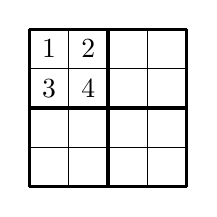
\begin{tikzpicture}[scale=.5]
\begin{scope}
    \draw (0, 0) grid (4, 4);
    \draw[very thick, scale=2] (0, 0) grid (2, 2);
    \setcounter{rowa}{1}
    \setrowa {1}{2}{}{}
    \setrowa {3}{4}{}{}
    \setrowa {}{}{}{}
    \setrowa {}{}{}{} 
  \end{scope}
\end{tikzpicture}
\caption{B1 standardised}
\label{fig:shidokurelabelling}
\end{figure}

Next set the values for B2 $\cap$ R1. This must be a permutation of $\{3,4\}$, there exists 2! permutations. $x_a = 2\times x_b$. The same applied for B3 $\cap$ C1, we permute the set $\{2,4\}$. 

\begin{eqnarray}x_b &= 2\times x_c\\ x_c &=2\times x_d\end{eqnarray}
\begin{figure}[h]
\centering
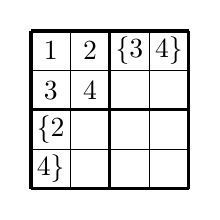
\begin{tikzpicture}[scale=.5]
\begin{scope}
    \draw (0, 0) grid (4, 4);
    \draw[very thick, scale=2] (0, 0) grid (2, 2);
    \setcounter{rowa}{1}
    \setrowa {1}{2}{\{3}{4\}}
    \setrowa {3}{4}{}{}
    \setrowa {\{2}{}{}{}
    \setrowa {4\}}{}{}{} 
  \end{scope}
\end{tikzpicture}
\caption{Permutations}
\label{fig:shidokurelabelling}
\end{figure}

The final stage is easy enough to brute force. Observe there exists only three ways to complete the remaining cells.

\begin{figure}[h]
\centering
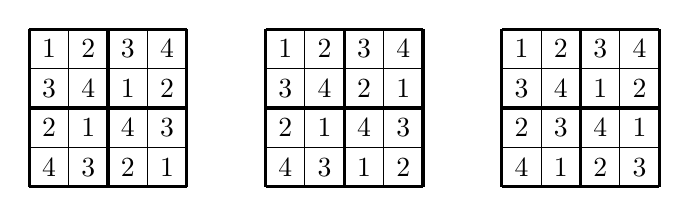
\begin{tikzpicture}[scale=.5]
\begin{scope}[xshift=0cm]
    \draw (0, 0) grid (4, 4);
    \draw[very thick, scale=2] (0, 0) grid (2, 2);
    \setcounter{rowa}{1}
    \setrowa {1}{2}{3}{4}
    \setrowa {3}{4}{1}{2}
    \setrowa {2}{1}{4}{3}
    \setrowa {4}{3}{2}{1} 
  \end{scope}
\begin{scope}[xshift=6cm]
    \draw (0, 0) grid (4, 4);
    \draw[very thick, scale=2] (0, 0) grid (2, 2);
    \setcounter{rowa}{1}
    \setrowa {1}{2}{3}{4}
    \setrowa {3}{4}{2}{1}
    \setrowa {2}{1}{4}{3}
    \setrowa {4}{3}{1}{2} 
  \end{scope}
\begin{scope}[xshift=12cm]
    \draw (0, 0) grid (4, 4);
    \draw[very thick, scale=2] (0, 0) grid (2, 2);
    \setcounter{rowa}{1}
    \setrowa {1}{2}{3}{4}
    \setrowa {3}{4}{1}{2}
    \setrowa {2}{3}{4}{1}
    \setrowa {4}{1}{2}{3} 
  \end{scope}
\end{tikzpicture}
\caption{Three Complete Shidokus}
\label{fig:shidoku}
\end{figure}

This completes the enumeration, we have $x_4=4!\times 2 \times 2 \times 3 = 288$. 

Observe that the last three shidokus squares are not in fact unique, we can transform the second to the third. 

\begin{figure}[h]
\centering
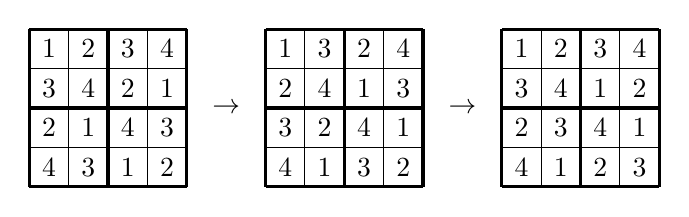
\begin{tikzpicture}[scale=.5]
\begin{scope}
    \draw (0, 0) grid (4, 4);
    \draw[very thick, scale=2] (0, 0) grid (2, 2);
    \setcounter{rowa}{1}
    \setrowa {1}{2}{3}{4}
    \setrowa {3}{4}{2}{1}
    \setrowa {2}{1}{4}{3}
    \setrowa {4}{3}{1}{2} 
\end{scope}
\node[anchor=center] at (5, 2) {$\rightarrow$};
\begin{scope}[xshift=6cm]
    \draw (0, 0) grid (4, 4);
    \draw[very thick, scale=2] (0, 0) grid (2, 2);
    \setcounter{rowa}{1}
    \setrowa {1}{3}{2}{4}
    \setrowa {2}{4}{1}{3}
    \setrowa {3}{2}{4}{1}
    \setrowa {4}{1}{3}{2} 
  \end{scope}
\node[anchor=center] at (11, 2) {$\rightarrow$};
\begin{scope}[xshift=12cm]
    \draw (0, 0) grid (4, 4);
    \draw[very thick, scale=2] (0, 0) grid (2, 2);
    \setcounter{rowa}{1}
    \setrowa {1}{2}{3}{4}
    \setrowa {3}{4}{1}{2}
    \setrowa {2}{3}{4}{1}
    \setrowa {4}{1}{2}{3} 
  \end{scope}
\end{tikzpicture}
\caption{Transformation}
\label{fig:shidokutransformation}
\end{figure}

Ultimately, we only have two completely unique shidokus. One of these shidokus has 192 others equivalent and the other 96 this can be seen from the final step of our enumeration, three shidokus are found each wiith 96 corresponding equivalents but we can reduce three to two combining the equivalents. This shows the amount of equivalent shidokus is dependent on the shidoku square and not all symmetries produce a valid shidoku that hasnt been seen before.

We have answered two interesting questions about shidoku through a singular analysis however this will not apply for the larger cases. Let us generalise the use of symmetries and equivlance relations into a way to count our truely unique shidokus.

\noindent\rule{4cm}{0.4pt}

\textbf{Unique}

Let us take a group theory approach. We define a Shidoku Symmetry as a map from the set of Shidoku boards to itself. There is two type which we shall explore. Relabeling symmetries, $x\mapsto y$, change the labels within the shidoku so that all cells with label $x$ change to $y$, set $R_4$ defines all such symmetries. Structural symmetries describe movements of cells, there are many such moves so we shall define possible symmetries and then condense these into the necessary minial generators of this set. We name the set $S_4$. Our entire set of symmetries is formed from the cartesian product of these sets as we can combine them to get further symmetries (as seen above where we transform a sudoku using a reflection and a relabeling), $G_4=S_4\times R_4$.

Which manipulations of the cells within the Shidoku board map to another valid shidoku board? 
\begin{itemize}
\item Swap R1 and R2,
\item swap R3 and R4,
\item swap C1 and C2,
\item swap C3 and C4,
\item swap S1 and S2,
\item permute P1 and P2,
\item rotate the board 90$^\circ$ clockwise,
\item transpose the board (in the natural way, as though the board were a matrix).
\end{itemize}
Note these structural symmetries are neither extensive (we could include further rotations) nor minimal (swapping C1 and C2 can be achieved by rotating, swapping R1 and R2 then rotating 3 more times). Denoting $s$ as the swap of R3 and R4, $r$ the 90$^\circ$ clockwise rotation and $t$ the transpose, we can generate $H_4$ through these.

\begin{equation}H_4 = \langle s,r,t | e=s^2=r^4=t^2\rangle\end{equation}

We then get $G_4$ to be of order $128\times 4!=3072$. However this is much larger than the set of shidoku boards. We note from our previous analysis the largest set of equivalent shidokus is of size 192. This suggests we can find a smaller $G_4$ group as its minimum possible size is 192. \cite{} explores the possible minimal groups in detail we will summarise them here for completeness see \ref{table:group}. Finding a minimal symmetry group is not just satisfying but it is useful. We greatly reduce the computation required for our next step.

\begin{table}[!h]
\begin{center}
\begin{tabular}{ |c|c|c| }
 \hline
Group & Order & Orbits\\
 \hline
 $\langle r,t \rangle \times S_4$ & 192 & 5\\
 $\langle r,s \rangle \times S_4$ & 1536 & 2\\
 $\langle r,s \rangle \times \langle (123)\rangle$ & 192 & 2\\
 $\langle s,t \rangle \times S_4$ & 192 & 2\\
 $H_4 \times\langle (123) \rangle $ & 384 & 2\\
 $\langle r^2,s,t \rangle \times \langle (123) \rangle$ & 192 & 2\\
 \hline
\end{tabular}
\end{center}
\caption{\label{table:group}Groups, Order and Orbits}
\end{table}

\textbf{Burnside's Lemma:} For a thorough overview of this result see \cite{analysis and applications of burnsides lemma jenny jin}, an account and analysis that this author found very useful. For a finite group $G=G_4$ acting on the set $S$ of shidoku boards we have $S/G_4$ denoting the set of orbits of $S$. 
\begin{equation} |S/G_4|=\frac{1}{|G_4|}\sum_{g\in G_4}|S^g|\end{equation}
where $|S^g|$ is the set of all elements in $S$ that are unchanged by element $g$ acting upon it. In english this means we can count the orbits of the shidoku symmetries acting on the set of shidoku boards (how many distinct shidokus exist) by calculating the avergae of the boards left unchanged by each element of the symmetry group. 

Now we are going to change our idea of invariance a bit but it will not change its underlying meanin, only how we interact with it and use it in this context. We can view all elements of the symmetry group as a structual symmetry action followed by a relabling action so a board $s\in S$ is invariant if for $g\in S_4$ and $h\in H_4$, $h(g(s))=s$ or $g(s)=h^{-1}(s)$ as $H_4 $ is a group, $h^{-1}\in H_4$. So with the maths asside we can observe invariance through the lens of just the structural symmetries. A shidoku board $b\in S$ if invariant under structural symmetry $x$ if there exists a  relabeling symmetry $r\in R_4$ such that $r$ can undo the action $x$.

Obsereve we minimise calculations by choosing a minimal symmetry group (order 192) and as our invariance concept allows focus on the structural symmetries we minimise this to. So we choose to use $\langle s,t \rangle \times S_4$ from \ref{table:groups}.

Another way to minimise calcultions is to find conjugacy classes, as for conjugacy class C if $a\in C$ and $a$ is invariatn, that is there exists $r\in R_4$ such that$ra(B)=B$ then all elements conjugate to a such that $b=gag^{-1}$ for $g\in H_4$ are also invairnat. We get this from teh following, note elements of $R_4$ commute with elements of $H_4$ and from ra(B)=B, $r=a^{-1}$:
\begin{eqnarray}
rb(B)&=&rgag^{-1}(B)\\
&=&grag^{-1}(B)\\
&=&geg^{-1}(B)\\
&=&gg^{-1}(B)\\
&=&e(B)\\
&=&B
\end{eqnarray}
We have five conjugacy classes so we only check five symmetries for invariance. 

We can prove invariance by considering fixing relationships between structure and relabeling. 

\textbf{The Fixing Lemmas}: If b in S is invariant under x via r then:
\begin{itemize}
\item Value: if a cell location is unchanged under x having value n, r must map $n \mapsto n$.
\item Region: if all cells in a block, sash or pillar are unchanged under x then r is the identity relabeling. 
\item Fixed Point: if r maps $n\mapsto n$ the x must the subset of cells with value n to the same subset.
\end{itemize}
These are easy to verify through observation but if you require a solid proof go to \cite{minimal complete shidoku symmetry groups pg 10}.

We have all we need to calculate the Burnside Lemma table \ref{table:burnside}. A brief discussion: as s fixes R1 and R2 this cannot be invariant as the fixing lemmas suggest r would be the identity relabeling but $s(b)\neq b$; stst fixes B1 so the same reasoning applies and st ... As for t, the relabelling must be such that the main diagonal in B1 remains the same (so 1 and 4 are unchanges when the standardised B1 configuration is used) and the other two cells in B1 are flipped ($2\mapsto 4$). Observe in \ref{fig:transpose} there are only two shidoku squares that are invariant under a transpose and the proposed relabeling. The identity element of course preserves all shidoku boards.

\begin{figure}[h]
\centering
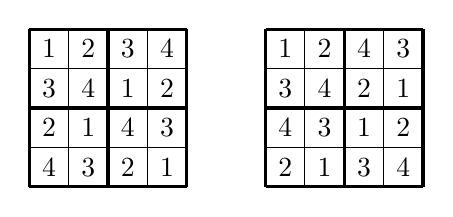
\begin{tikzpicture}[scale=.5]
\begin{scope}[xshift=0cm]
    \draw (0, 0) grid (4, 4);
    \draw[very thick, scale=2] (0, 0) grid (2, 2);
    \setcounter{rowa}{1}
    \setrowa {1}{2}{3}{4}
    \setrowa {3}{4}{1}{2}
    \setrowa {2}{1}{4}{3}
    \setrowa {4}{3}{2}{1} 
  \end{scope}
\begin{scope}[xshift=6cm]
    \draw (0, 0) grid (4, 4);
    \draw[very thick, scale=2] (0, 0) grid (2, 2);
    \setcounter{rowa}{1}
    \setrowa {1}{2}{4}{3}
    \setrowa {3}{4}{2}{1}
    \setrowa {4}{3}{1}{2}
    \setrowa {2}{1}{3}{4} 
  \end{scope}
\end{tikzpicture}
\caption{These shidoku are invariant under $t$, $2\mapsto 3$}
\label{fig:transpose}
\end{figure}

\begin{table}[!h]
\begin{center}
\begin{tabular}{ |c|c| }
 \hline
Class  & No. of Invariant boards\\
 \hline
$C_e=\{e\}$&$12\times 4!$\\
$C_s = \{s,tst\}$&0\\
$C_t = \{t,sts\}$&$2\times4!$\\
$C_{st}=\{st,ts\}$&0\\
$C_{stst}=\{stst\}$&0\\
\hline
\end{tabular}
\end{center}
\caption{\label{table:burnside}}
\end{table}

Now we finally apply the Burnside lemma to give:
\begin{equation}|S/G_4|=\frac{1(12\times 4!)+ 2(0)+2(2\times 4!)+2(0)+1(0)}{8\times 4!}=2.\end{equation}
To prove what we already knew! Not amazing but at least we get the point and can use these techniques for larger boards.

The main issue here of course is fining a minimal symmetry group, luckily this paper addresses it \cite{minimal complete shidoku symmetry groups} through considering the structural and relabeling symmetries separately as we have determined is a helpful technique. We will not discuss this further as we must move on to bigger but not necessarily better sudokus.

	\section{$6 \times 6$}
	
\noindent\rule{4cm}{0.4pt}
\textbf{How many?}

We follow a similar strategy to count our rudoku boards, however the literature on this is limited and this author provides the enumeration calculations. 

The first move is alwasy the easiest, we standardise B1. Reducing our search space by 9!.  $x_6=9!\times x_a$

Our R1 will be seperated into two cases coined pure and mixed. A pure R1 consists of B1 $\cap$ R2 in a single box (B2 $\cap$ R1 or B3 $\cap$ R1) and B1 $\cap$ R3 in the other. A mixed, like the name suggests has B2 $\cap$ R1 as an amalgamation of B1's R2 and R3. The pure case is simple, the first row consists of set $\{3,4\}$ $\{5,6\}$ which forces the sets in R2 and R3. Our count is therefore $2^6$ for the different permutations of these sets multipled by 2 as B2 and B3 can be permuted. $2^7=128$

Mixed takes more consideration. R1 must be a permutation of sets has two choices $\{\{3,5\},\{4,6\}\}$ or $\{\{3,6\},\{4,5\}\}$. This forces 5,6 to be in R2 and 3,4 into R3 leaving 1,2 to be placed. Counting these decisions we get 2 for where we put 1 (forcing 2), 2 for which R1 set we take, 2 to flip B2 and B3 then $2^6$ to permute each of the sets. Overall we have $2\times 2 \times 2 \times 2^6=2^9=512$. 

S1 has $2^9+2^7=640$ possible completions. We now must count how many S2 completions there are for each board, call this $b_i$.

\begin{equation}x_a = \sum^{640}_{i=1}b_i\end{equation}

This will take a lot of computation power so let's simplify this further. Observe a completion of S1 has the same $b_i$ as the same completion of S1 but with B2 and B3 flipped, currently we compute this twice but this is a waste. We expand this idea further to permutation of R3-4 and R5-6. This means each board in the 640 completions has $2\times 2\times 2$ boards that are equivalent when columns and boxes are permuted. This limits the search space to $\frac{640}{8}=80$. In practise this means we do not allow some of teh choices described above. For the pure case we set R1 to be 1,2,3,4,5,6 leaving only $2^4=16$ choices. Then for the mixed we set R1 to be 1,2,3,5,4,6 or 1,2,3,6,4,5 leaving $2^5$ choices left and remember the choice between these two R1s so we get $2^6=64$. 

\begin{equation}x_a=8\sum^{80}_{i=1}b_i\end{equation}

There is still work to be done, for all 80 boards we must compute $b_i$. Lets do a brief approximation currently that would mean there for each column in S2 there are three possible numbers this gives $3!^6 = 46656$ possible solutions that need to be checked. We can reduce this further by a factor of 3!. For C1 $\cup$ S2 set 2,4,6, not this has 3! permutations each of which have the same amount of completions as the board with forced C1. So we redefine $b_i$ count only solutions with C1 1,3,5,2,4,6.

\begin{equation}x_6=9!3!8\sum^{80}_{i=1} b_i\end{equation}

From my own computation $\sum^{80}_{i=1} b_i=816$. \footnote{The source code can be found at https://github.com/EveRoutledge/sudoku, the code is in python and yet still runs in under a minute.}

Finally we have $x_6=28200960$. This does not look promising, there is a massive difference from $x_4=288$. This number has been calculated but without detailed account of method. 

\noindent\rule{4cm}{0.4pt}

\textbf{Unique}

Already we are becoming too large
Leading on from 4 by 4 approach
possible symmetries
\begin{itemize}
\item Swap R1 and R2,
\item swap R2 and R3,
\item Swap R4 and R5,
\item swap R5 and R6,
\item swap C1 and C2,
\item swap C3 and C4,
\item swap C5 and C6
\item swap S1 and S2,
\item swap P1 and P2,
\item swap P2 and P3,
\item rotate the board 180$^\circ$,
\item transpose the board (in the natural way, as though the board were a matrix).
\end{itemize}
no transpose
no flip
leads to less efficiencies
equivalence 
fixing lemmas
order of the group
conjugacy classes
GAP 

49
	\section{$9 \times  9$}

Now it is time to tackle the big one. The 9 by 9 sudoku is the largest board size for which enumerations have been widely discussed with this author only finding one website discussing the 10 by 10 case. Similarly enumerations for the latin square stop at 11. Chapter 2 explored theoretical exponential increase in difficulty when sudoku boards increase in size and we have seen it in action throughout this chapter. A generalised and efficient enumeration method seems unlikely but is certainly fun to try so let us continue to our final enumeration.

\textbf{How many?}

We start as usual by standarising B1. This shrinks the search space by a factor of 9!. Then our usual technique takes place, find all possible S1 configurations, group them into sets that will have the same amount of completions for S2 and S3 then brute force the completions with an optimised algorithm.

To calculate the amount of possibilities for S1 we examine the pure and mixed case. The pure case uses the set  in B1 $\cup$ R2 ($\{4,5,6\}$) in either B2 $\cup$ R1 or B3 $\cup$ R1 and B1 $\cup$ R3 ($\{7,8,9\}$) in the other. This forces the sets in the other rows of S1. Counting these we get $3!^6$ for the permutations of each set and as we can switch P2 and P3 we multiply by two. There are $2\times 3!^6$ pure cases of S1. 

The mixed case is a little more complicated. We first list the possible R1 $\cup$ B2 $\cup$ B3 options, see table \ref{table:mixed99}. This will set three values in the second and three in the third row leaving $\{1,2,3\}$ to be placed in the remaining cells. See diagram... Counting these we get $3\times3!^6$ for each configuration of the top row. Finally there are $9\times 2$ top row configurations from the table selecion and by swapping the P2 and P3. 

\begin{table}[!h]
\begin{center}
\begin{tabular}{ |c|c| }
 \hline
B2$\cup$R1  & B3$\cup$R1\\
 \hline
$\{4,5,7\}$&$\{6,8,9\}$\\
$\{4,5,8\}$&$\{6,7,9\}$\\
$\{4,5,9\}$&$\{6,7,8\}$\\
$\{4,6,7\}$&$\{5,8,9\}$\\
$\{4,6,8\}$&$\{5,7,9\}$\\
$\{4,6,9\}$&$\{5,7,8\}$\\
$\{5,6,7\}$&$\{4,8,9\}$\\
$\{5,6,8\}$&$\{4,7,9\}$\\
$\{5,6,9\}$&$\{4,7,8\}$\\
\hline
\end{tabular}
\end{center}
\caption{\label{table:mixed99}}
\end{table}

In total there are
\begin{equation}2\times3!^6+18\times 3\times 3!^6 = 2612736\end{equation}
S1 configerations with the standardised B1. This is an unreasonably large search space so we must reduce this like we have done previously through equivalence relations to discover which boards will have have the same amount of completions. 

Let us explore a few reductions.

\textbf{Column Permutations}
Observe boards with different permutations of C4-6 have the same number of completions (see \ref{fig:equiv99}). This is expanded to permutations of C7-9 and B2-3. Therefore from a single board we can derive $3!\times3!\times2=72$ other boards that are essentially equivalent. Our search space becomes $\frac{2612736}{72}=36288$, better but not ideal.

\begin{figure}[h!]
\centering
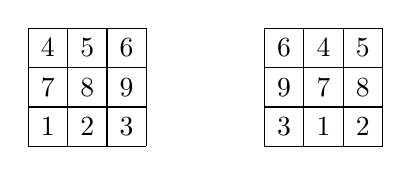
\begin{tikzpicture}[scale=.5]
\begin{scope}[xshift=0cm]
    \draw (0, 0) grid (3, 3);
    \setcounter{rowb}{1}
    \setrowb {4}{5}{6}
    \setrowb {7}{8}{9}
    \setrowb {1}{2}{3}
  \end{scope}
\begin{scope}[xshift=6cm]
    \draw (0, 0) grid (3, 3);
    \setcounter{rowb}{1}
    \setrowb {6}{4}{5}
    \setrowb {9}{7}{8}
    \setrowb {3}{1}{2}
  \end{scope}
\end{tikzpicture}
\caption{\label{fig:equiv99}Two configurations of B2 which are essentially equivalent}
\end{figure}

\textbf{Optimised Column Permutations and Relabelling}
We have excluded B1 in our permutation above in order to preserve our standardised B1 labeling but note relabeling is a symmetry and we can still utilise this further to improve our search space ($r_1pr_2$). We permute C1-3, C4-6, C7-9 and B1-3 giving $3!\times 3!\times 3! \times 3!=1296$ possibly equivalent boards to be derived from a single board. We then we can relabel the new boards to again standardise B1. From \cite{}enumerating possible sudoku grids, page 4 we note this reduces the search space to 2051 boards. If each board had exactly 1296 equivalent boards we would have $\frac{2612736}{1296}= 2016$ boards in our search space \textbf{why dont we}.  We now have to catalog the amount of boards corresponding to each of the 2051 as, unlike the previous reduction, this reduction does not affect all boards equally.

\textbf{Permutations of S1 Rows}
Taking a leaf out of the Optimised Column Permutations and Relabelling book we can apply this to the rows of sash 1. We do this by permuting the rows and relabeling B1 to it's standardised form. This gives each board another the possibility of having $3!$ more equivalent boards now giving a grand maximum of $1296\times 3!=7776$ eqivalent boards, of course this is not the case for every board as we discussed, otherwise we could have had a search space of $\frac{2612736}{7776}=336$ but we are not far off with the reduction coming out at 416 (from \cite{}enumerating possible sudoku grids, page 4).

\textbf{Reducing Twins}
Twins are two values in C$n$ lying in R$x$ and R$y$ such that the values also lie in C$m$ in R$x$ and R$y$ where $n\neq m$. For example figure \ref{fig:twins} has values 1 and 4 in R1, R2, C1, C4. By the relabeling $1\mapsto 4$, $4\mapsto 1$ we get another board with the same amount of completions, that is to say the complete S2,3 are independent of the lables 1 and 4. This gives us another equivalence reduction. From \cite{}enumerating possible sudoku grids, page 5 we reduce the 416 equivalence classes to 174.

\begin{figure}[h!]
\centering
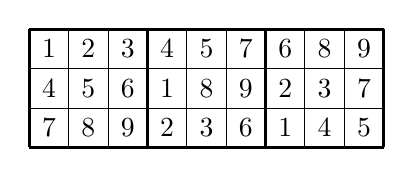
\begin{tikzpicture}[scale=.5]
\begin{scope}[xshift=0cm]
    \draw (0, 0) grid (3, 3);
\draw[very thick, scale=3] (0, 0) grid (3, 1);
    \setcounter{rowb}{1}
    \setrowb {1}{2}{3}
    \setrowb {4}{5}{6}
    \setrowb {7}{8}{9}
  \end{scope}
\begin{scope}[xshift=3cm]
    \draw (0, 0) grid (3, 3);
    \setcounter{rowb}{1}
    \setrowb {4}{5}{7}
    \setrowb {1}{8}{9}
    \setrowb {2}{3}{6}
  \end{scope}
\begin{scope}[xshift=6cm]
    \draw (0, 0) grid (3, 3);
    \setcounter{rowb}{1}
    \setrowb {6}{8}{9}
    \setrowb {2}{3}{7}
    \setrowb {1}{4}{5}
  \end{scope}
\end{tikzpicture}
\caption{\label{fig:twins}}
\end{figure}

Observe this can be expanded to larger subsets, see figure \ref{}. This uses 3 columns. and figure \ref{} uses 4 columns with the values 1,5. Again from \cite{} this reduces us to 71 classes. see mathematics of sudoku I for in depth

\begin{figure}[h!]
\centering
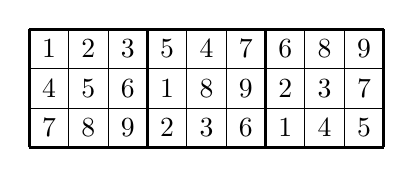
\begin{tikzpicture}[scale=.5]
\begin{scope}[xshift=0cm]
    \draw (0, 0) grid (3, 3);
\draw[very thick, scale=3] (0, 0) grid (3, 1);
    \setcounter{rowb}{1}
    \setrowb {1}{2}{3}
    \setrowb {4}{5}{6}
    \setrowb {7}{8}{9}
  \end{scope}
\begin{scope}[xshift=3cm]
    \draw (0, 0) grid (3, 3);
    \setcounter{rowb}{1}
    \setrowb {5}{4}{7}
    \setrowb {1}{8}{9}
    \setrowb {2}{3}{6}
  \end{scope}
\begin{scope}[xshift=6cm]
    \draw (0, 0) grid (3, 3);
    \setcounter{rowb}{1}
    \setrowb {6}{8}{9}
    \setrowb {2}{3}{7}
    \setrowb {1}{4}{5}
  \end{scope}
\end{tikzpicture}
\caption{\label{fig:twins}}
\end{figure}

\begin{figure}[h!]
\centering
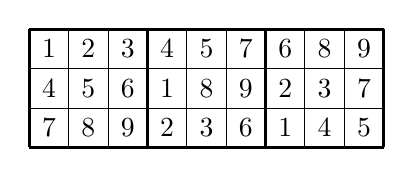
\begin{tikzpicture}[scale=.5]
\begin{scope}[xshift=0cm]
    \draw (0, 0) grid (3, 3);
    \draw[very thick, scale=3] (0, 0) grid (3, 1);
    \setcounter{rowb}{1}
    \setrowb {1}{2}{3}
    \setrowb {4}{5}{6}
    \setrowb {7}{8}{9}
  \end{scope}
\begin{scope}[xshift=3cm]
    \draw (0, 0) grid (3, 3);
    \setcounter{rowb}{1}
    \setrowb {4}{5}{7}
    \setrowb {1}{8}{9}
    \setrowb {2}{3}{6}
  \end{scope}
\begin{scope}[xshift=6cm]
    \draw (0, 0) grid (3, 3);
    \setcounter{rowb}{1}
    \setrowb {6}{8}{9}
    \setrowb {2}{3}{7}
    \setrowb {1}{4}{5}
  \end{scope}
\end{tikzpicture}
\caption{\label{fig:twins}}
\end{figure}

Brilliant we have reduced our S1 to only 71 boards to search. However we still need to enumerate the solutions for each of these which is alot of searching and as we know from Chapter 2 finding a single solution isnt very efficient so counting how many exist is worse. Let us attempt to improve this. By using the exact same argument as S1 on P1 we get 2612736 completions which can be reduced to 36288 equivalence classes with 72 members. We can repeat the twins equivalence relation idea but \cite{} reason the search space ahs been reduced enough that the computation is feasible. 44 distinct counts.

For algorithmic details consult \cite{}. This paper states the number of valid sudoku grids is 6,670,903,752,021,072,936,960 6 sextillion. This has been corroborated by the first discover of this number by \cite{} lin keh ying.
 
 \noindent\rule{4cm}{0.4pt}
 
\textbf{Unique} 

Discuss symmetries
Equivalence definition as 4 by 4
group size
Conjugacy classes
Many classes have no equivalent grids
Burnside Lemma
Conclusion
Reflection not a symmetry for all sizes
Discuss GAP

5,472,730,538

\section{Verification}

Enumerating sudoku requires a computer to work through the laborious and trivial tasks described in this chapter. This is both a strength and a weakness of the computers place in modern mathematics. Previously this work would be enscribed in large notebooks by someone who enjoys monotonous work. Now hundreds of man hours become an hour of coding and pressing run. The improvement is mathematicians are freed up to explore new questions and leave the trivial to the machine but it also means there is a middle man between the mathematician and the answer, a middle man that may have created errors. Scepticism follows any computational proof, the pure nature of mathematics and logic sullied. This author, straddling the worlds of mathematics and computer science sees the merits of the machine but too feels the lack of satisfaction at the inelegance of the code. 

A famous example of the conflict between mathematics and the computer is the proof of the Four Colour Theorem. The Theorem states: a map requires no more than four colours to colour it in such a way that no adjacent regions have the same colour. The idea of the proof being the mathematicians reduced the map possibilities and a computer then exhausts all possible colourings to confirm each instance only requires four colours. The proof was controversial no person could feasibly check the computation \cite{swart1980philosophical}. The theorem has been proven three times\cite{appel1989every}\cite{BarNatan1996LieAA}\cite{gonthier2008formal}, all using a computer, the most recent of which uses software specifically designed to assist with proving theorems, much like the GAP software used for the sudoku proofs. 

The literature on enumertaion of sudokus answers this computer based scepticism with a complete mathematical proof outline in the works by Jones, Perkins and Roach \cite{mima2013number} where a formula is given to enumerate $n$ by $n$ sudokus by enumerating the number od reduced sudoku. Further work by Jones, Perkins and Roach \cite{jones2014number} provides a completely mathematical calculation of the $6\times6$ sudoku.

\section{Discussion}

If the reader remained unconvinced that sudoku is hard from the chapter on NP-completeness then this chapter providing concrete numbers on the exponential increase of the amount of sudoku grids will hopefully persuade the reader of the seemingly non generalisable puzzle that is sudoku. The sequence of enumerations starts: 288, 28200960, ..., 6670903752021072936960. Within the first four terms we have reached 6 sextillion. 

While it does not seem to be coming any time soon, an exploration of the 12 by 12 case will prove interesting as there exist two factorisations $P_{2,6}$ and $P_{3,4}$. The comparison between these and determining which has more enumerations is not intuitive and to shed light on this is intriguing. The same applied to the 16 by 16 place but with the added bonus we can compare a grid allowing for transposes the $P_{16}$ and one that does not $P_{2,8}$.

As far as a generalised method goes, first standardise B1, categorise R1 into pure and mixed, count how many S1 exist, standardise C1, then enumerate using an optimised backtracking. The unique case is a lot less simple and requires a categorisation of the symmetries, we then group into conjugacy classes, determine how many boards the conjugacy class fixes the apply burnside lemma, use of GAP can simplify this.

% ~~~~~~~~~~~~~~~~~~~~~~~~~~~~~~~~~~~~~~~~~~~~~~~~~~~~~~~~~~~~~~~~~~~~~~~~~~~~~~~~~~~~~~~~~~~~ %
\chapter{Further Work}

Solutions and enumerations of sudoku are not the only difficult and seemingly impossible to generalise questions within sudoku. Generation, Minimum clue to provide unique solution.

Orthogonal sudoku squares. uniqueness solution 

Information Theory application.
Grobner Basis
% ~~~~~~~~~~~~~~~~~~~~~~~~~~~~~~~~~~~~~~~~~~~~~~~~~~~~~~~~~~~~~~~~~~~~~~~~~~~~~~~~~~~~~~~~~~~~ %
\bibliographystyle{plain}
\bibliography{refs}
\end{document}
